\documentclass[main.tex]{subfiles}
\begin{document}

\chapter{Evaluation}

In diesem kapitel werden zuvor ausgewählte algorithmen einheitlich verglichen und die resultierenden ergebnisse ausgewertet.

\section{Evaluation Protocol}

To determine the feasibility of performing real-time plane detection, we need to conduct experiments with the selected algorithms.

Another important factor for comparability is the data set, on which the experiments are conducted on.
Because each publication from the presented algorithms uses a different data set for its evaluation, we cannot objectively select an algorithm to be the "best".
Furthermore, to the best of our knowledge, there is no data set, that contains an incrementally growing and unordered point cloud with corresponding ground truth.

Thus, we first evaluate the algorithms on a dataset while excluding the temporal component. We do this by performing plane detection on whole point clouds, rather than
incrementally growing ones.

We then perform experiments, this time including the temporal component, by performing calculations at each time step and evaluating them individually.

Lastly, through comparison, as well as analysis of those different experiments, a statement will be given as to whether and how well plane detection is
possible in real-time.

For the evaluation of a given dataset, by comparing the test results with the ground truth, we took inspiration from \citeauthor{Araújo_Oliveira_2020} \citedate{Araújo_Oliveira_2020},
especially their \textit{Results} chapter.


\subsection{Metrics}
To quantitatively evaluate an algorithm's performance, we calculate the precision, recall and the f1 score.
First, we regularize the original point cloud to reduce complexity and furthermore to avoid proximity bias, because of the inverse relationship
between distance to sensor and cloud density. This regularization is obtained through voxelization of the point cloud.\\
With this voxel grid, we can now calculate corresponding sets of voxels for each point cloud representing a plane.
In the next step, we compare our planes from the ground truth with the planes obtained from an algorithm to obtain a list of corresponding pairs
of ground truth and found planes.\\
A grund truth plane $p_{gt_i}$ is marked as \textit{detected}, if any plane from the list of found planes achieves a voxel overlap of $\geq 50\%$.
With this list of correspondences, we calculate precision, recall and the f1-score as explained in the following.
For a given ground truth plane $p_{gt_j}$ and a corresponding found plane $p_{a_k}$ we can sort a given voxel $v_i$ into the categories
\textit{True Positive(TP), False Positive(FP) and False Negative(FN)} as follows.
$$v_i \in p_{gt_j} \land v_i \in p_{a_k} \Rightarrow v_{i} \in TP$$
$$v_i \in p_{gt_j} \land v_i \notin p_{a_k} \Rightarrow v_{i} \in FN$$
$$v_i \notin p_{gt_j} \land v_i \in p_{a_k} \Rightarrow v_{i} \in FP$$
% TODO not needed right? $$v_i \notin p_{gt_j} \land v_i \notin p_{a_k} \Rightarrow v_{i} \in TN$$  , True Negative(TN)} 

With those four rules, we can calculate the precision, recall and F1 score like this:
$$Precision = \frac{|TP|}{|TP|+|FP|}$$
$$Recall = \frac{|TP|}{|TP|+|FN|}$$
$$F1 = 2 \cdot\frac{Precision\cdot Recall}{Precision + Recall}$$

Aside from the accuracy, we also need to compare the time each algorithm needs to find its respective set of planes.
For that, we measure the time spent in the plane detection phase, excluding any preprocessing or postprocessing steps.
To measure the detection time, we log the exact times before and after calculations and write the difference to a file.\\


\subsection{Dataset}
We select the Stanford Large-Scale Indoor Spaces 3D Dataset(S3DIS)\cite{2017arXiv170201105A} to evaluate each plane detection algorithm on even grounds.
S3DIS was recorded in three different buildings and divided into six distinct areas, including 272 different scenes. A detailed statistic of the included scene types can be found in Table~\ref{tab:stanfordStats}.
An individual scene has a complete unstructured point cloud and a list of annotated files representing semantically different objects that can be found therein.
Since our focus is not on 3D semantic segmentation, we manually select planar regions using CloudCompare\footnote{\href{https://cloudcompare.org/}{https://cloudcompare.org/}} to obtain a list of sub-clouds.

Furthermore, one could argue that an uneven distribution of scene types introduces a particular bias. While it is true that the distribution is quite uneven, the data set nevertheless reflects a realistic distribution of scene types since
it is not realistic that a building contains only lecture halls. On the other hand, it is appropriate to assume that an office complex contains a substantial amount of hallways needed to connect all these offices.

\begin{table}[!ht]
    \centering
    \begin{tabular}{c|c|c|c|c|c|c|c}
        \hline
        Scene Categories & Area\_1 & Area\_2 & Area\_3 & Area\_4 & Area\_5 & Area\_6 & TOTAL \\ \hline
        office           & 31      & 14      & 10      & 22      & 42      & 37      & 156   \\ \hline
        conference room  & 2       & 1       & 1       & 3       & 3       & 1       & 11    \\ \hline
        auditorium       & -       & 2       & -       & -       & -       & -       & 2     \\ \hline
        lobby            & -       & -       & -       & 2       & 1       & -       & 3     \\ \hline
        lounge           & -       & -       & 2       & -       & -       & 1       & 3     \\ \hline
        hallway          & 8       & 12      & 6       & 14      & 15      & 6       & 61    \\ \hline
        copy room        & 1       & -       & -       & -       & -       & 1       & 2     \\ \hline
        pantry           & 1       & -       & -       & -       & 1       & 1       & 3     \\ \hline
        open space       & -       & -       & -       & -       & -       & 1       & 1     \\ \hline
        storage          & -       & 9       & 2       & 4       & 4       & -       & 19    \\ \hline
        WC               & 1       & 2       & 2       & 4       & 2       & -       & 11    \\ \hline
        TOTAL            & 45      & 39      & 24      & 49      & 55      & 53      & 272   \\
    \end{tabular}
    \caption{S3DIS Disjoint Space Statistics}
    \label{tab:stanfordStats}
\end{table}

\subsection{Real-Life Test}
We record an incrementally growing data set in the Faculty of Computer Science at Otto-von-Guericke University Magdeburg.

Um den vergleich zwischen statisch und dynamisch noch besser zu gestalten, nehmen wir je einen dynamischen scene zu den folgenden scene typen aus S3DIS auf:
\begin{itemize}
    \item hallway
    \item office
    \item conferenceroom
    \item storage
    \item auditorium
    \item lobby
\end{itemize}
Wir nehmen keinen datensatz in WCs, copy rooms und storages auf, da die in der fin zu klein sind, um sich darin zu bewegen zu können. Ferner nehmen wir keinen
datensatz zu lounge auf, da sich das im kontext der fin nicht von einer lobby unterscheiden würde, open spaces gibt es nicht.

Running \textit{realsense-ros} and holding our cameras, we walk through different parts of the building, scanning to the best of our ability.
We save each incremental map update to a file for later usage.

We create a set of ground truth planes $gt_{end}$ for only the most recent update, e.g., for the entire recording.

To prepare for the evaluation of a map $m_t$ at a given time $t$, we crop all planes in $gt_{end}$ by removing all points that are not present in $m_t$, as shown in
Figure~\ref{fig:dynGT}.
We speed up this expensive process by employing a KD-Tree neighbor search with a small search radius since we only need to know whether a certain point is present or not.
Furthermore, we remove planes from the ground truth, if the number of included points falls short of a threshold.

\begin{figure}[H]
    \centering
    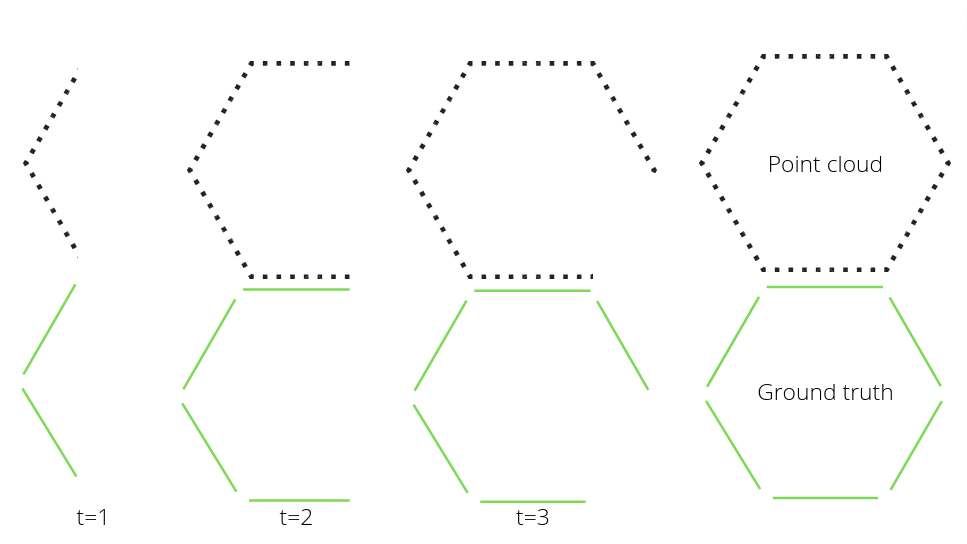
\includegraphics[width=15 cm]{images/dynamic_eval.png}
    \caption[Dynamic Ground Truth Generation]{Dynamic ground truth generation. All planes that are included in \textit{Ground Truth} are cropped depending on
        the available point cloud at each time \textit{t} }
    \label{fig:dynGT}
\end{figure}


\section{Results}

\subsection{Area 1}
\begin{figure}[H]
	\centering
	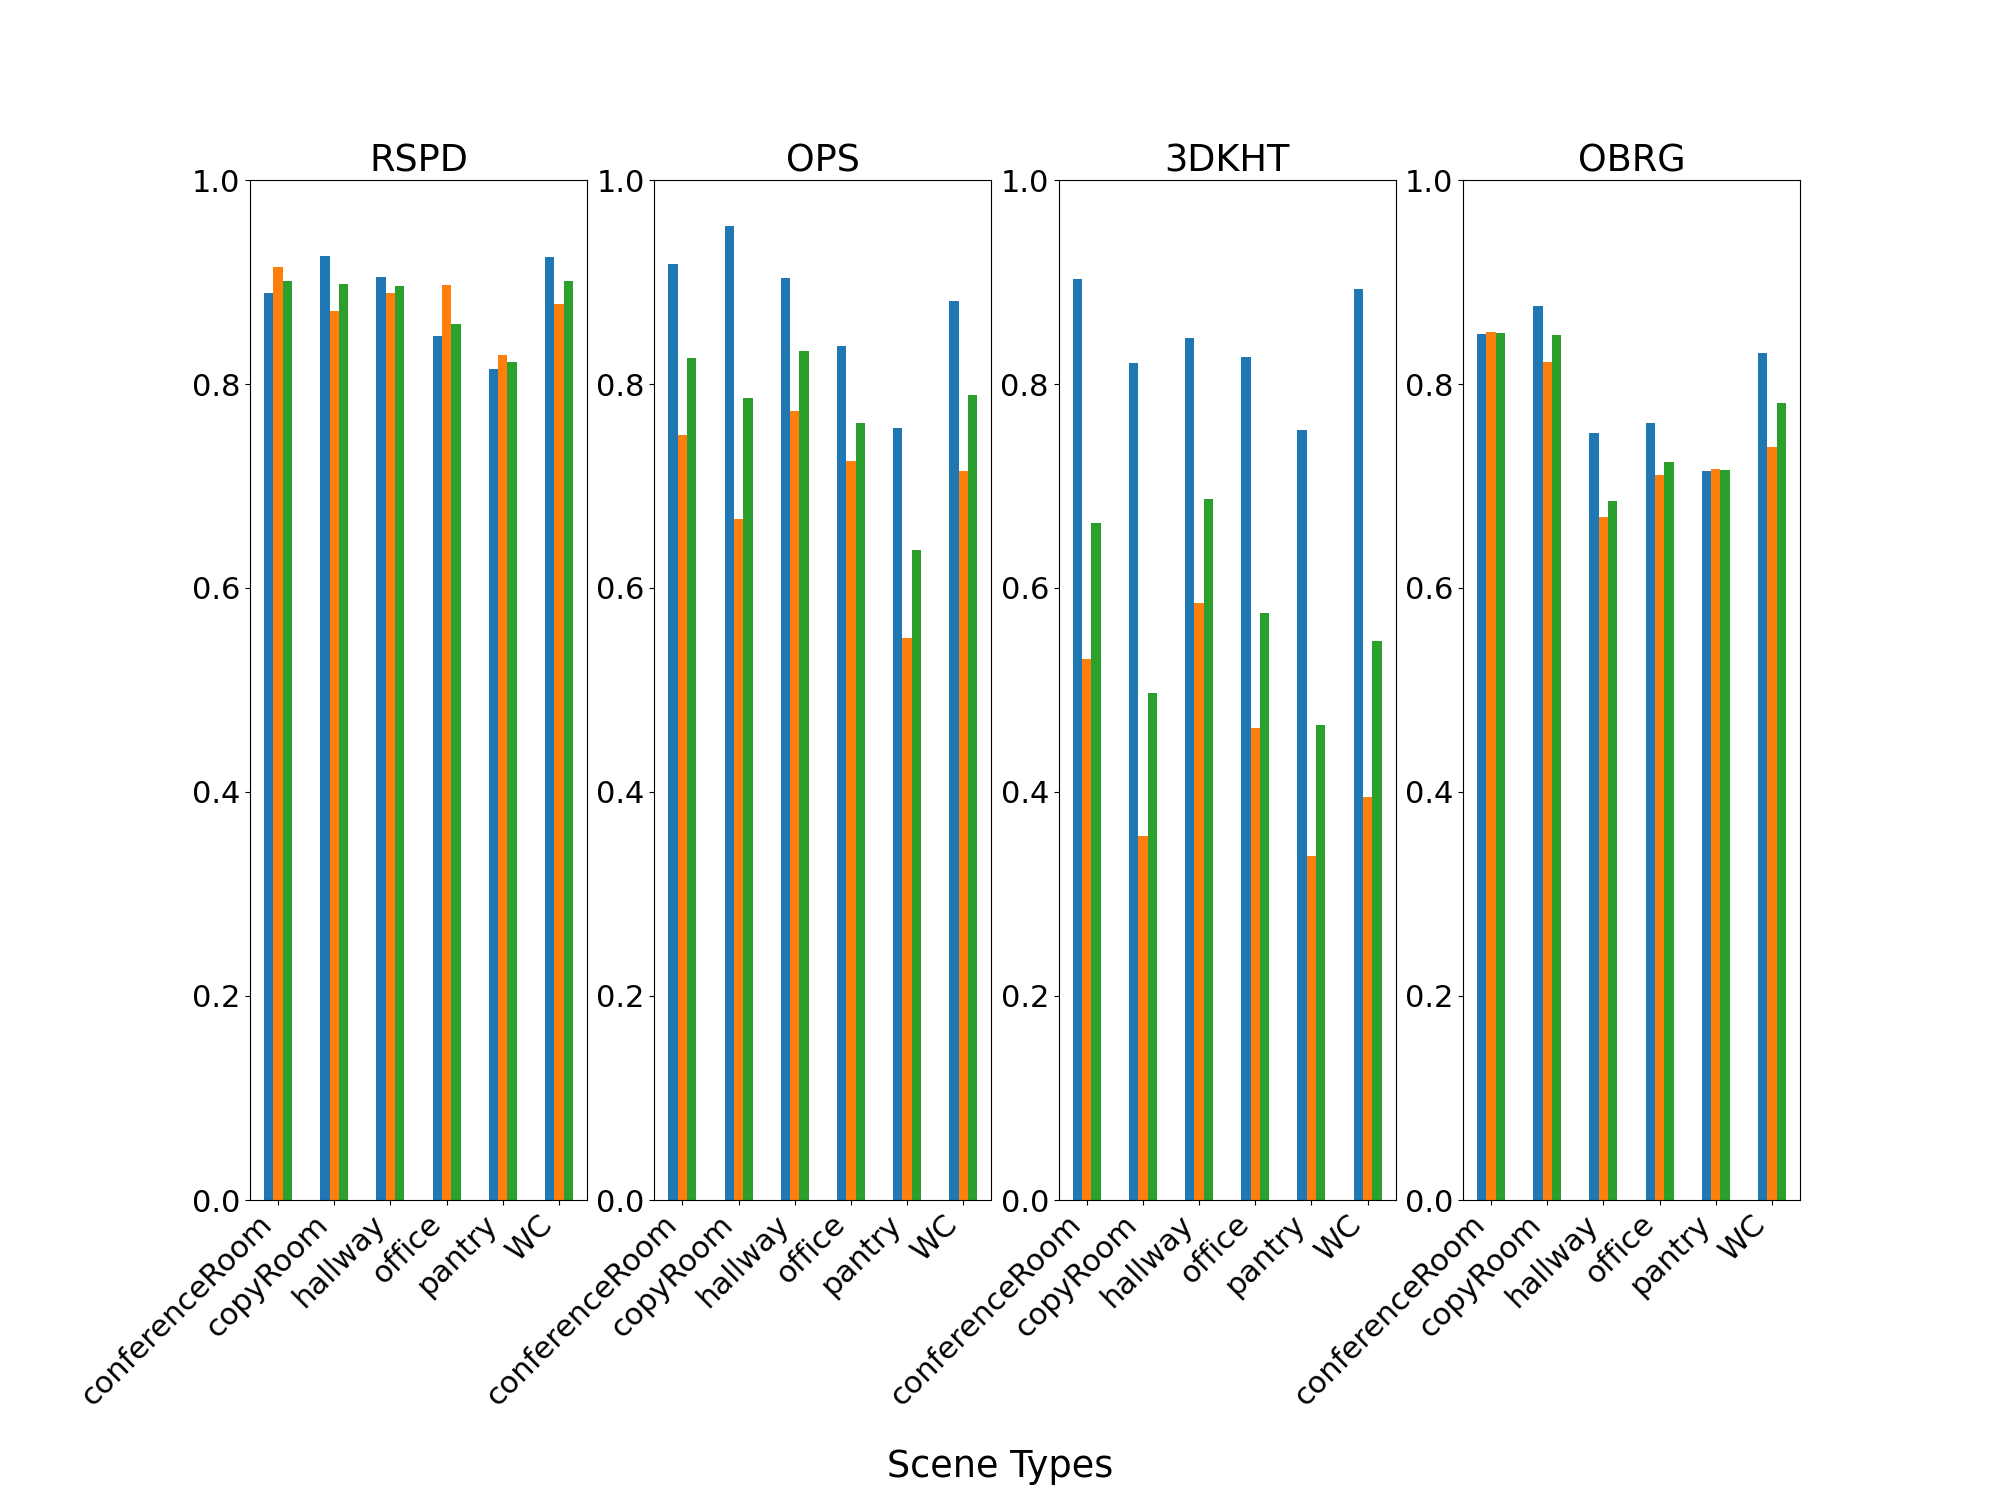
\includegraphics[width=15 cm]{images/area_1_acc.png}
	\label{fig:area1A}
    \caption[Accuracies Area 1]{Average Accuracy for each scene type of Area 1. The Precision 
    is colored blue, recall is orange and the F1-score is green. }
\end{figure}

\begin{figure}[H]
    \centering
	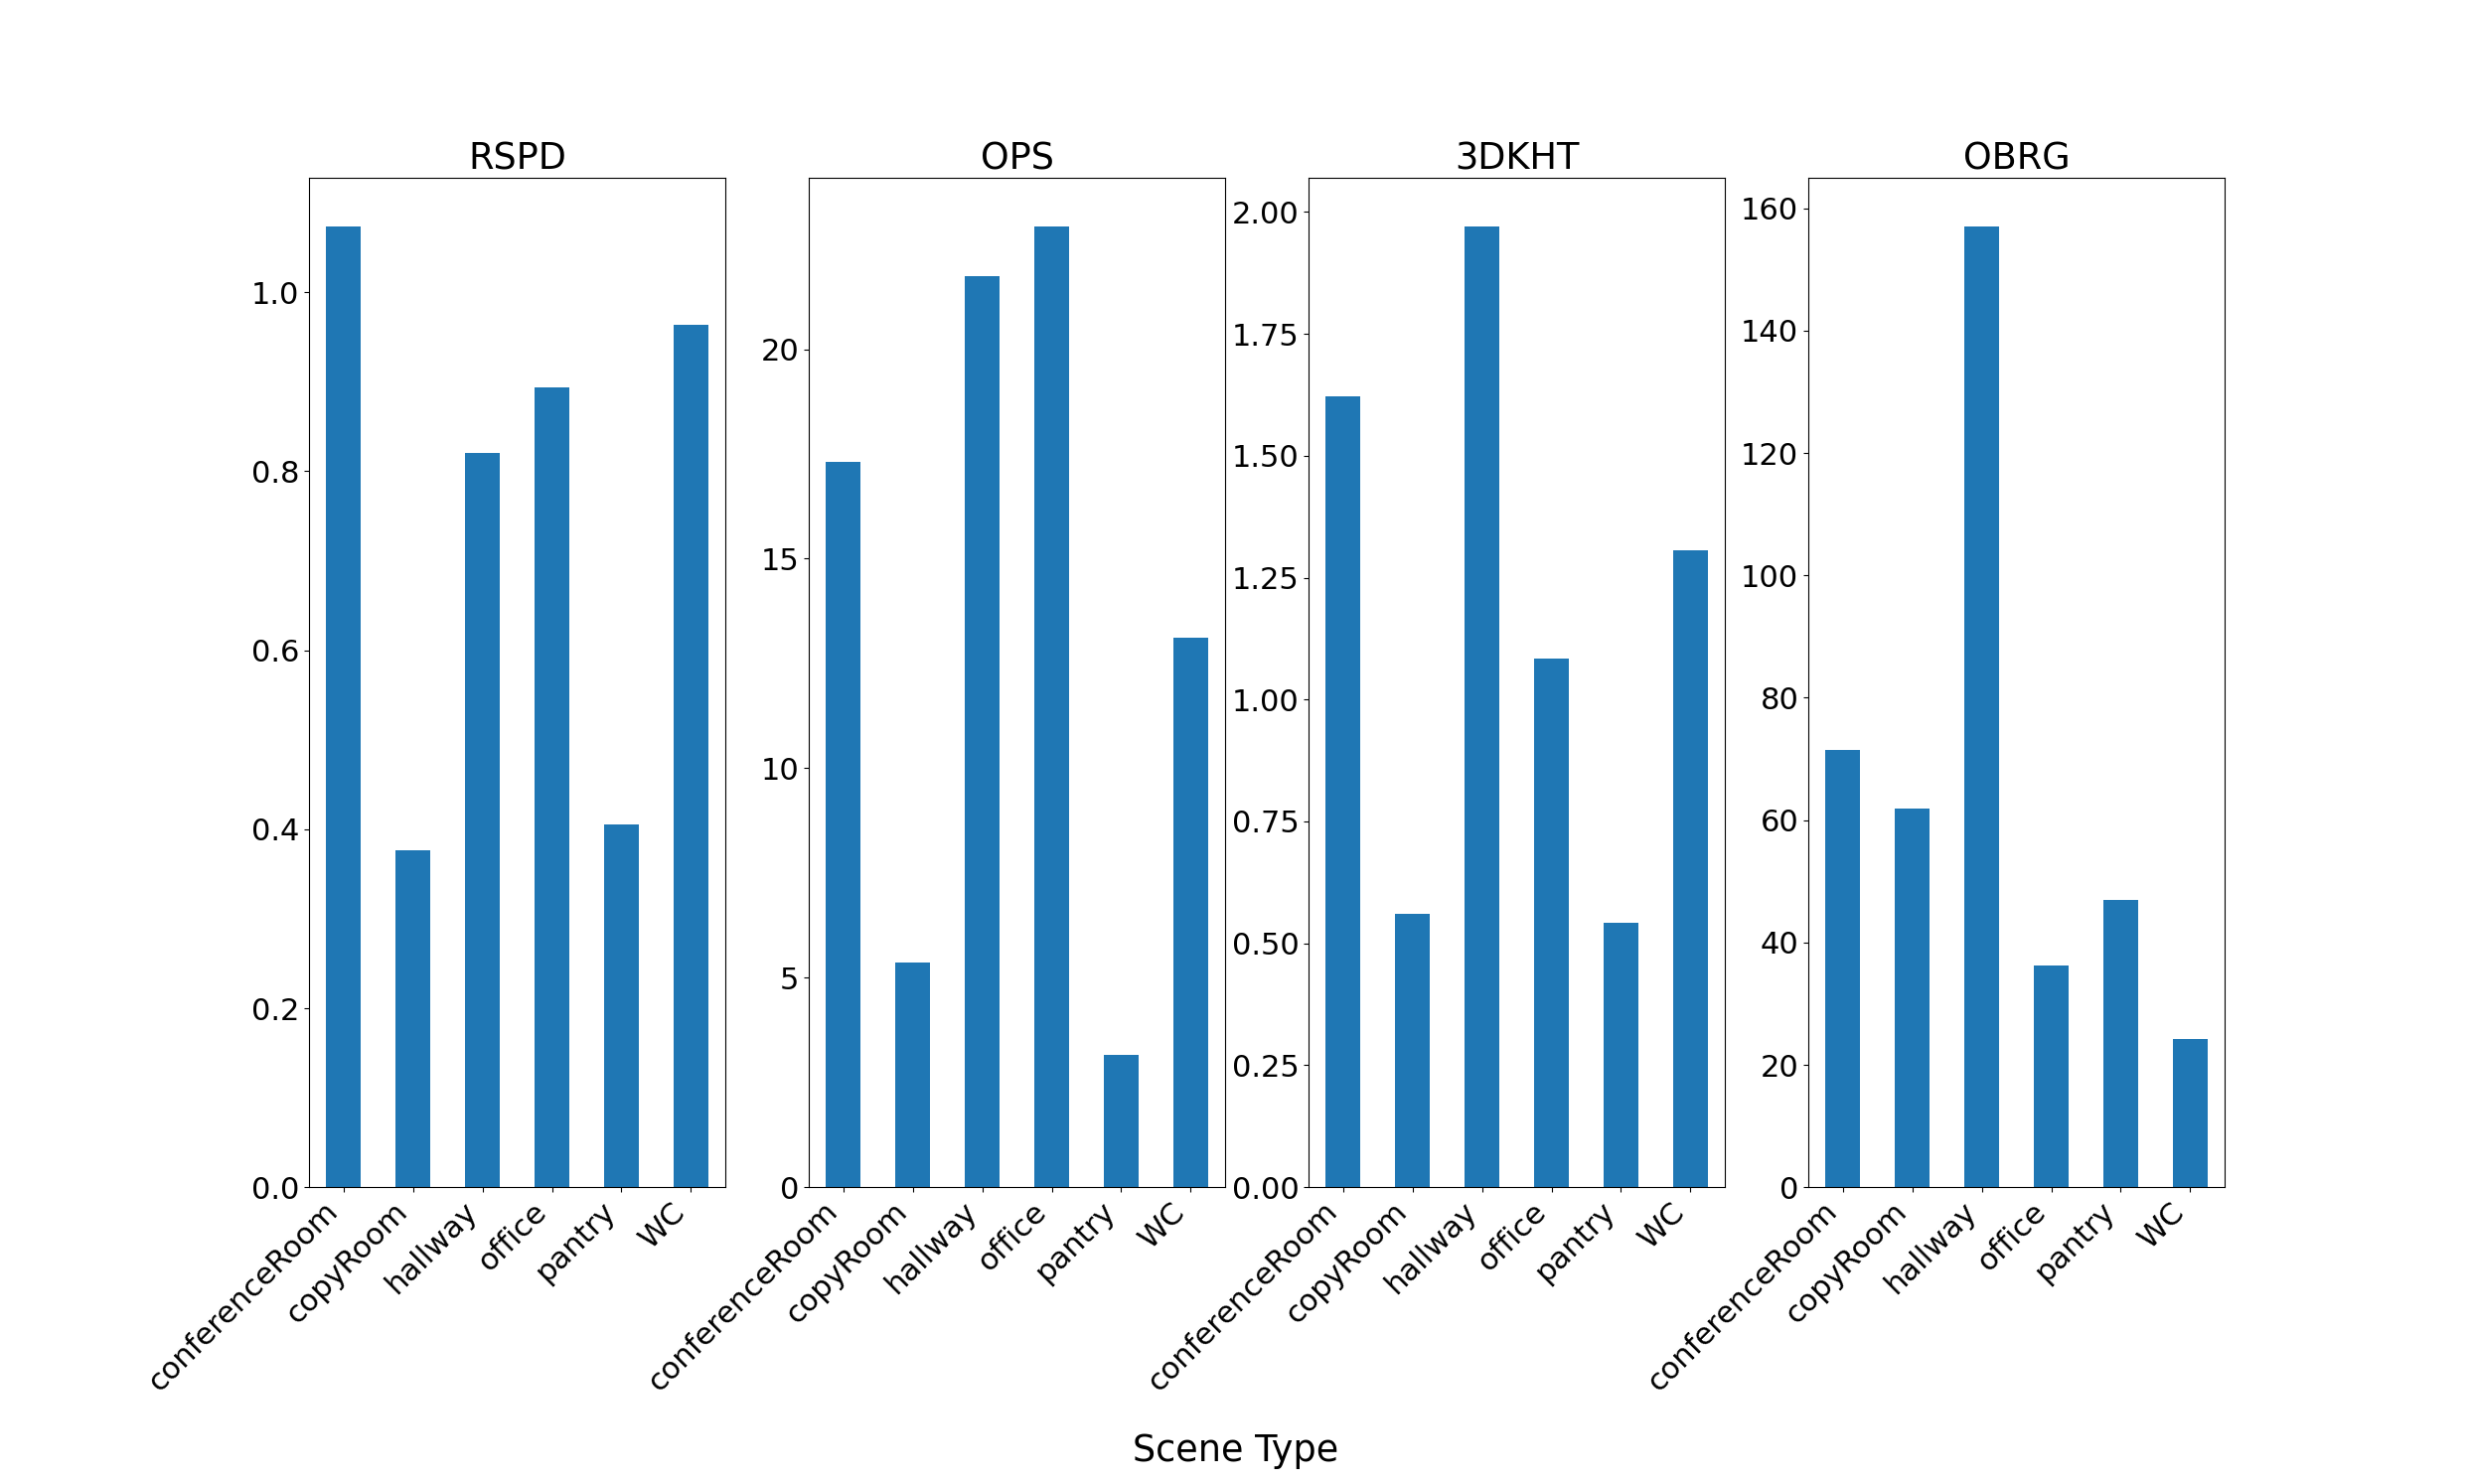
\includegraphics[width=15 cm]{images/area_1_time.png}
	\label{fig:area1T}
    \caption[Times Area 1]{Average Time per scene type of Area 1}
\end{figure}


\subsection{Area 2}

\begin{figure}[H]
    \centering
    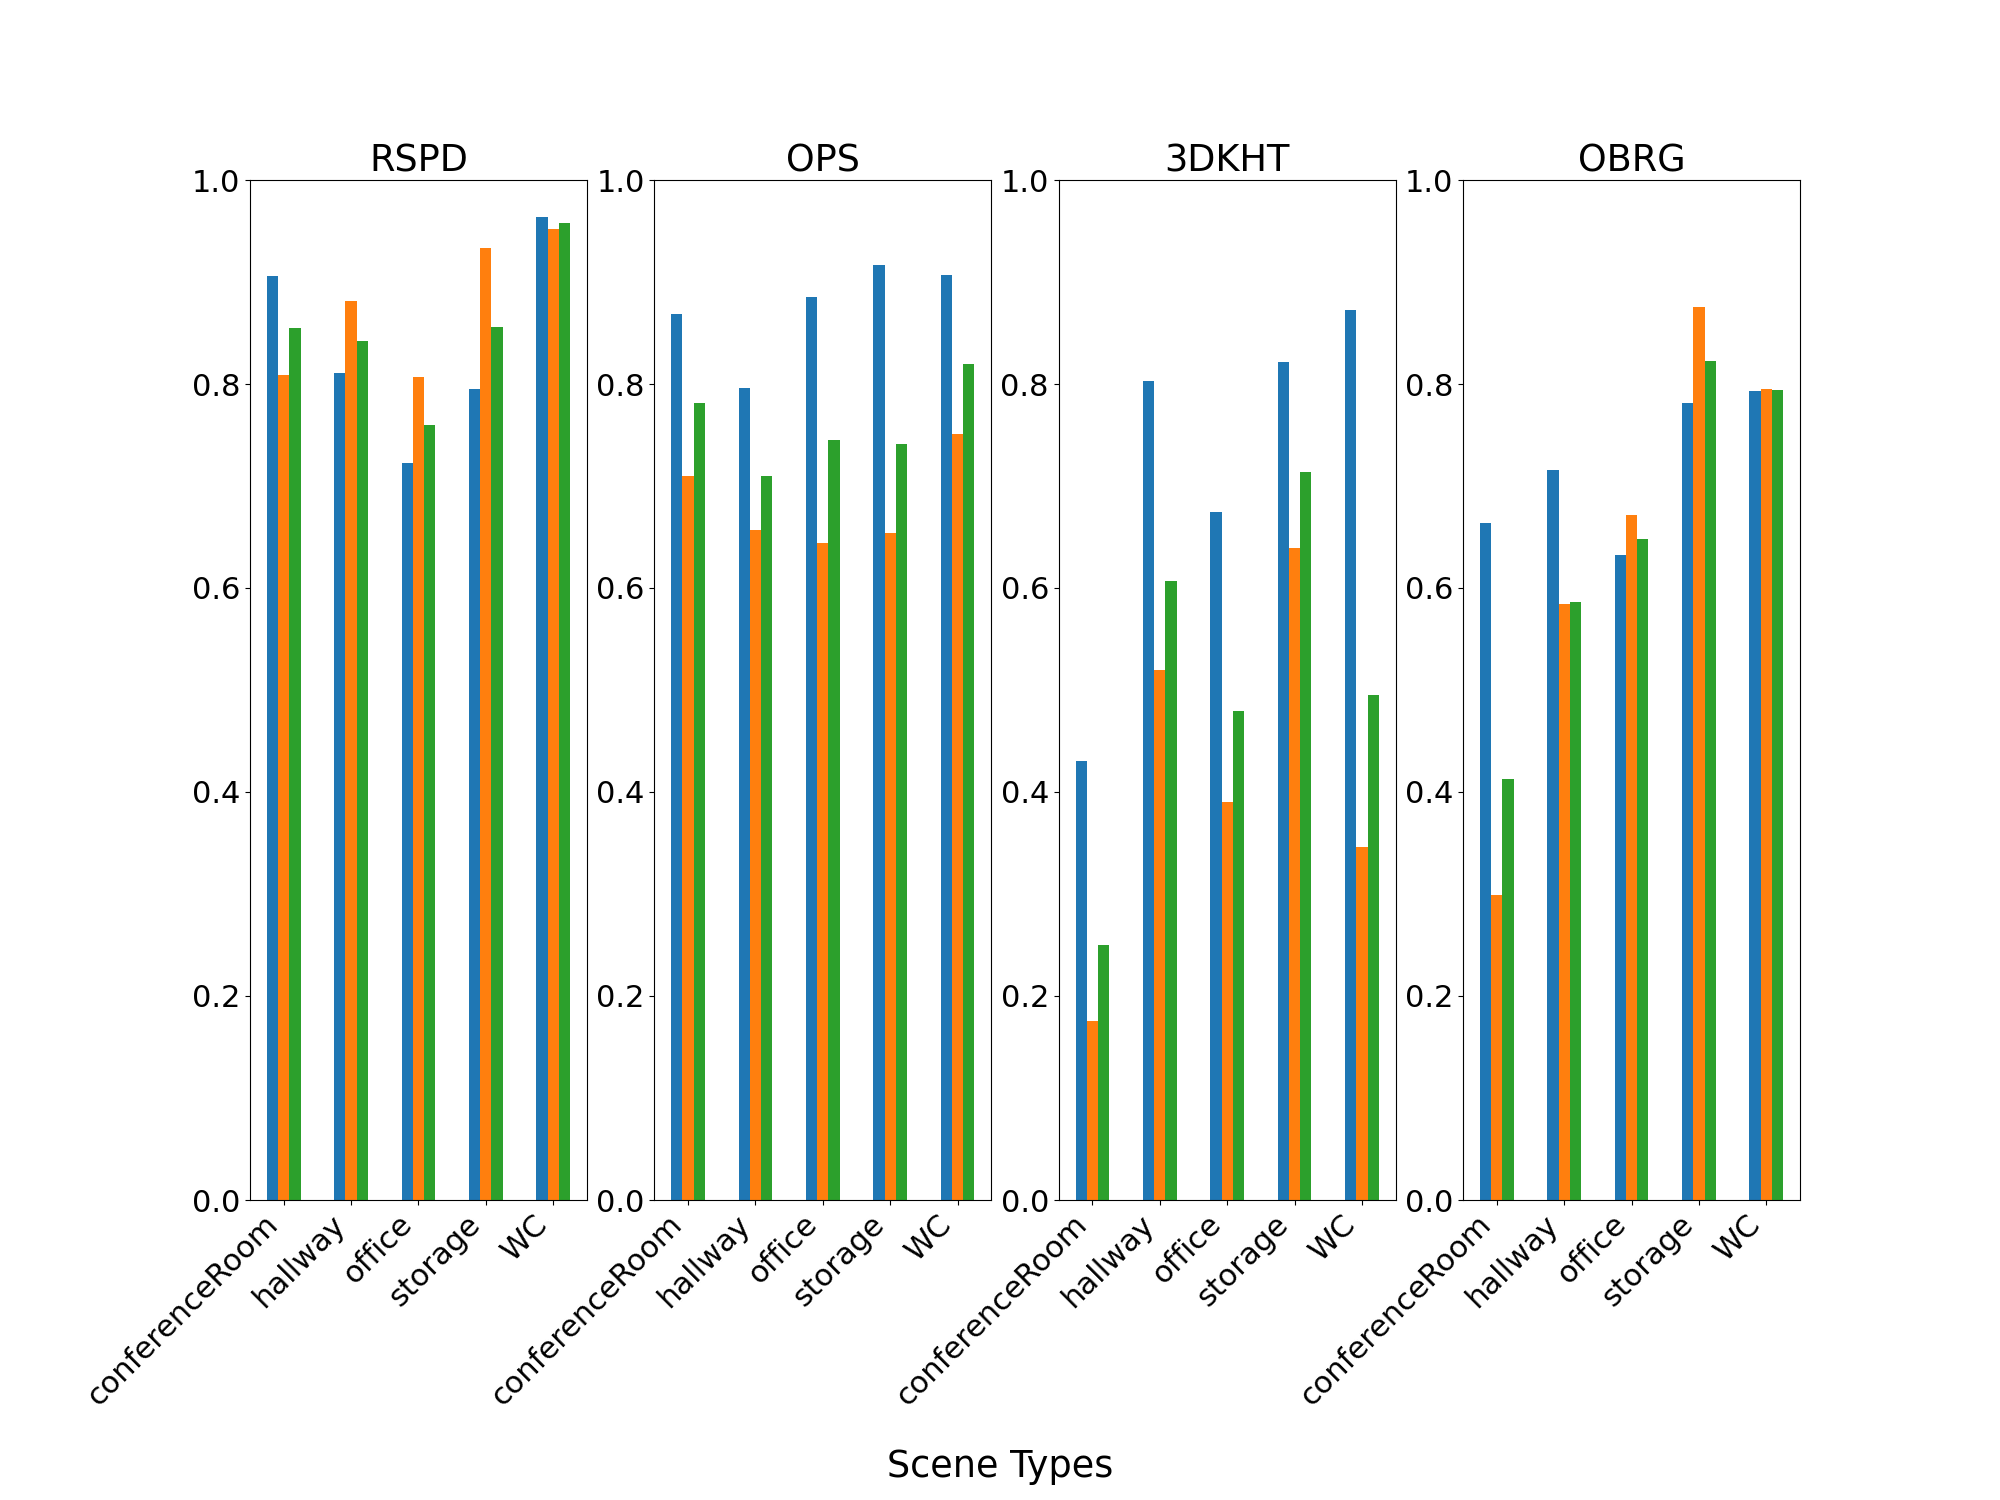
\includegraphics[width=15 cm]{images/area_2_acc.png}
    \caption[Accuracies Area 3]{Average Accuracy for each scene type of Area 2. The Precision
    is colored blue, recall is orange and the F1-score is green. }
    \label{fig:area2A}
\end{figure}

\begin{figure}[H]
    % FIXME normalize times 
    \centering
    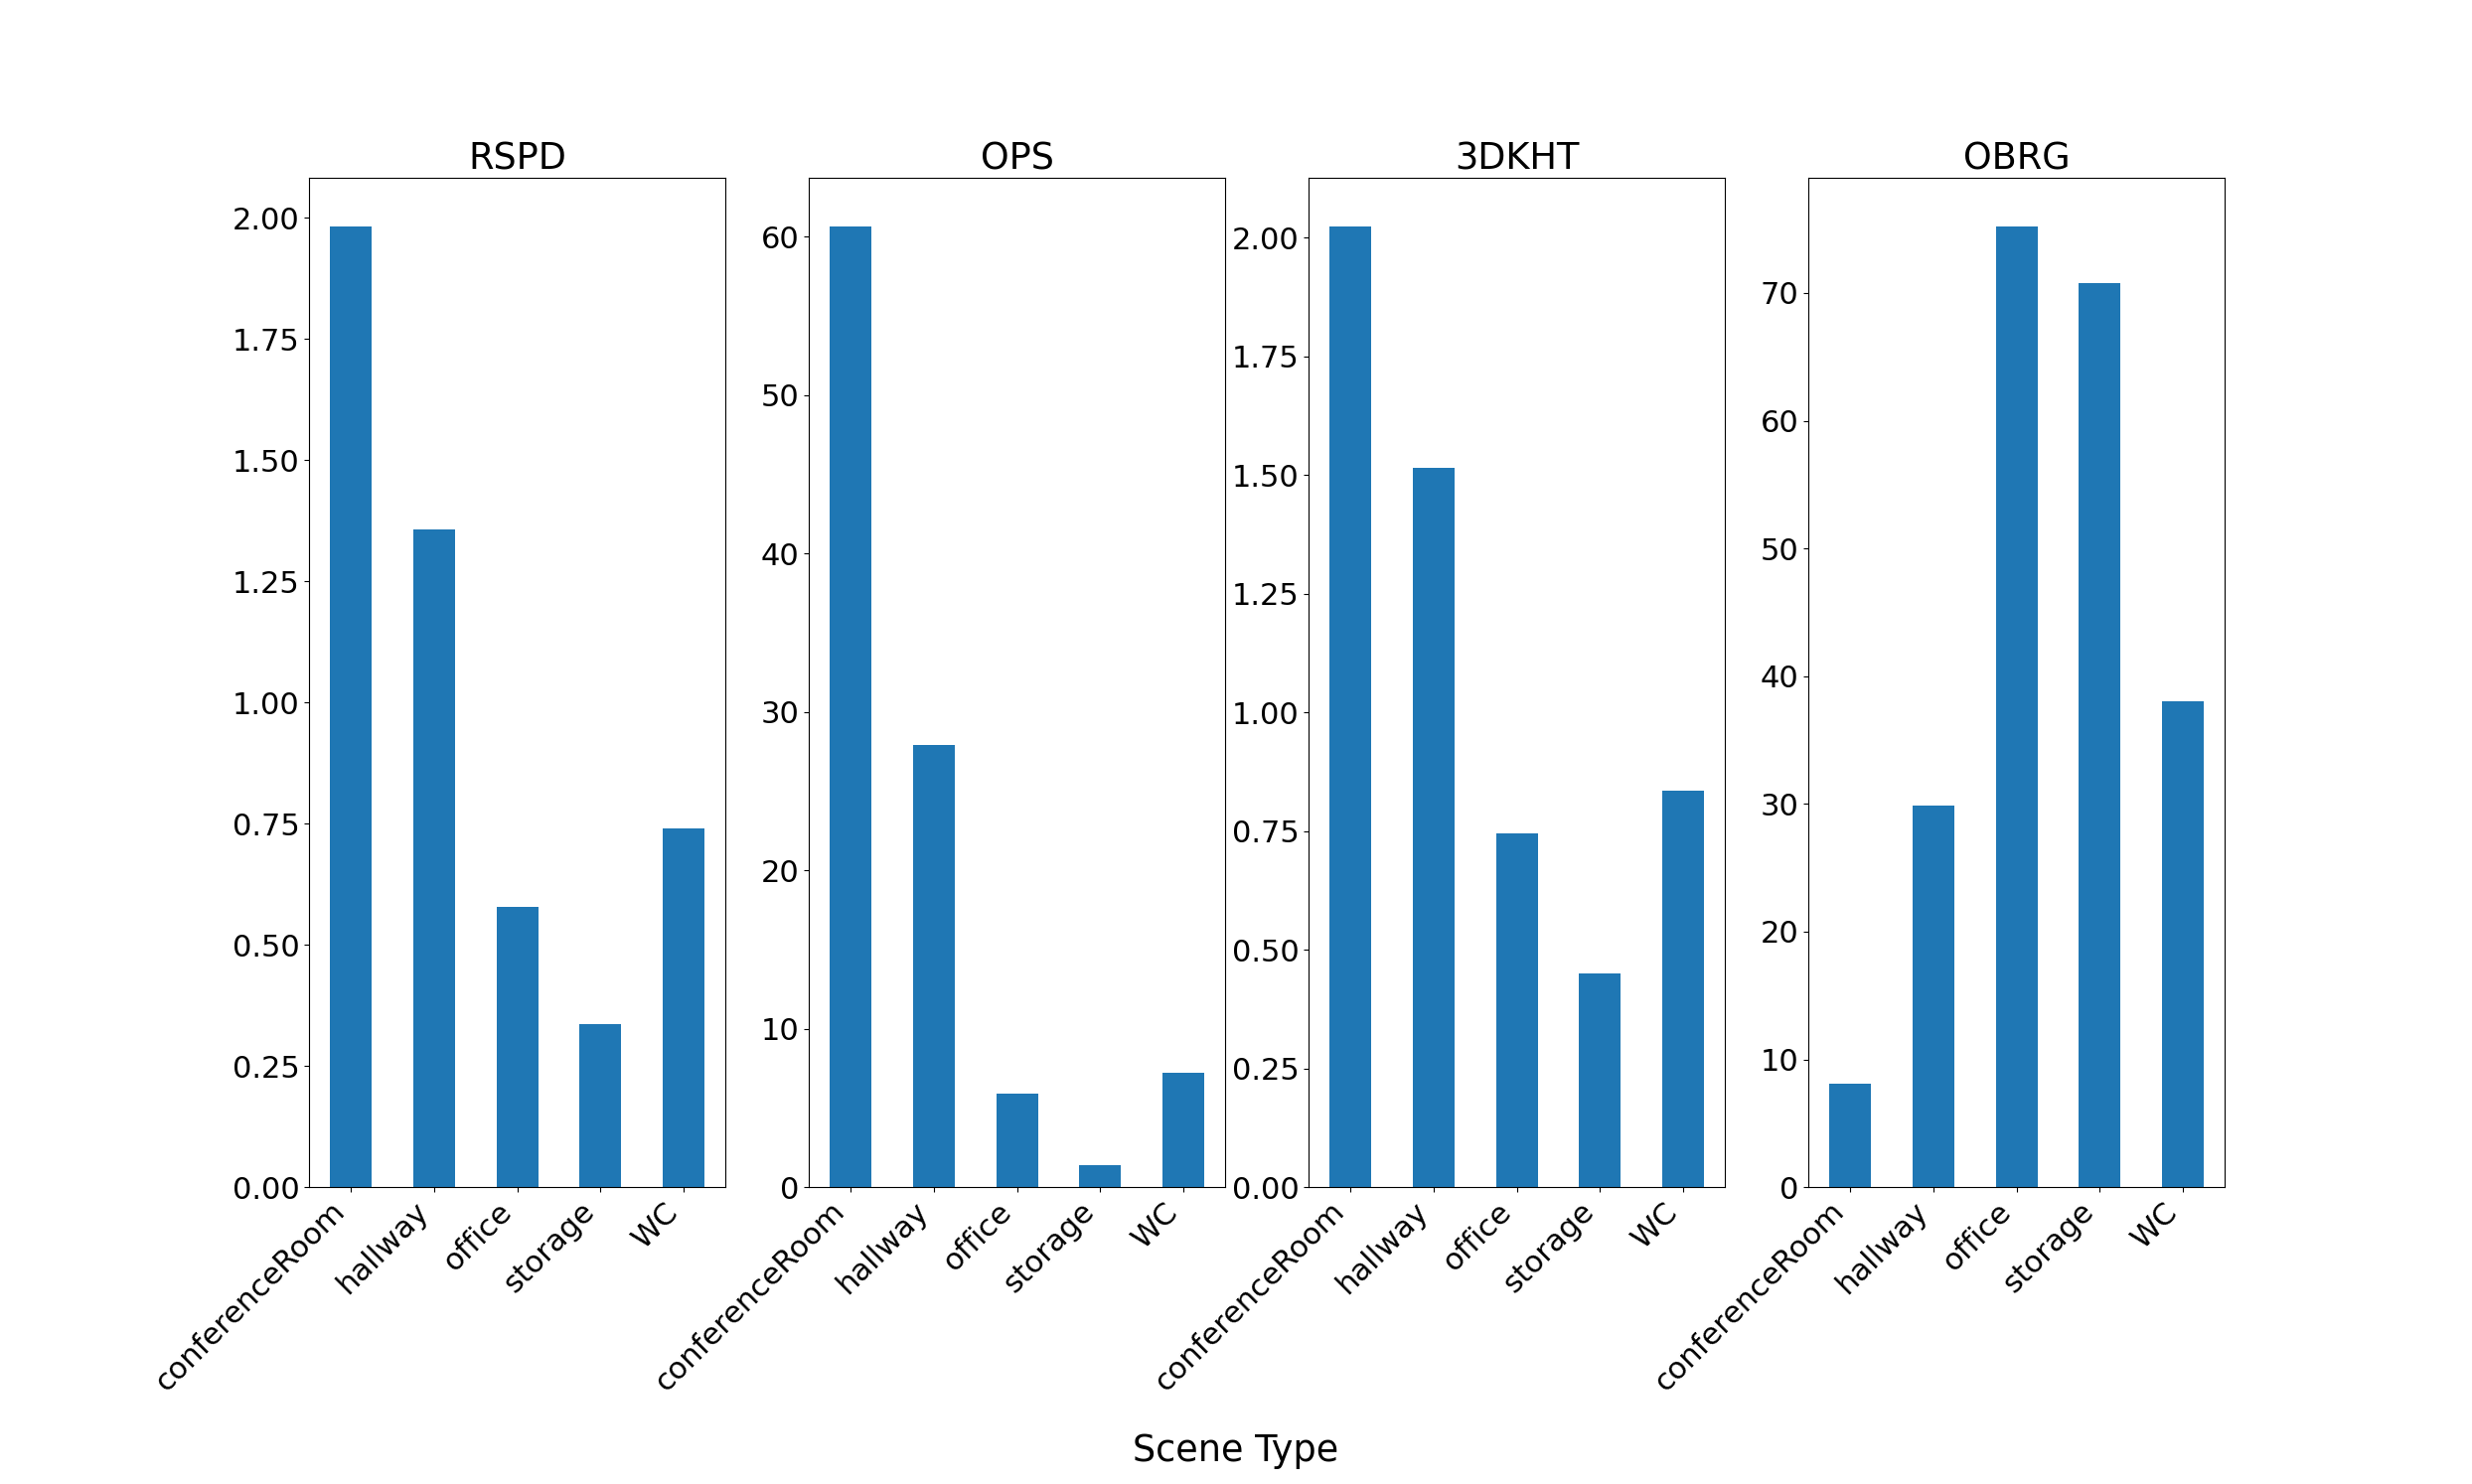
\includegraphics[width=15 cm]{images/area_2_time.png}
    \label{fig:area2T}
    \caption[Times Area 2]{Average Time per scene type of Area 2}
\end{figure}

\subsection{Area 3}

\begin{figure}[H]
    \centering
    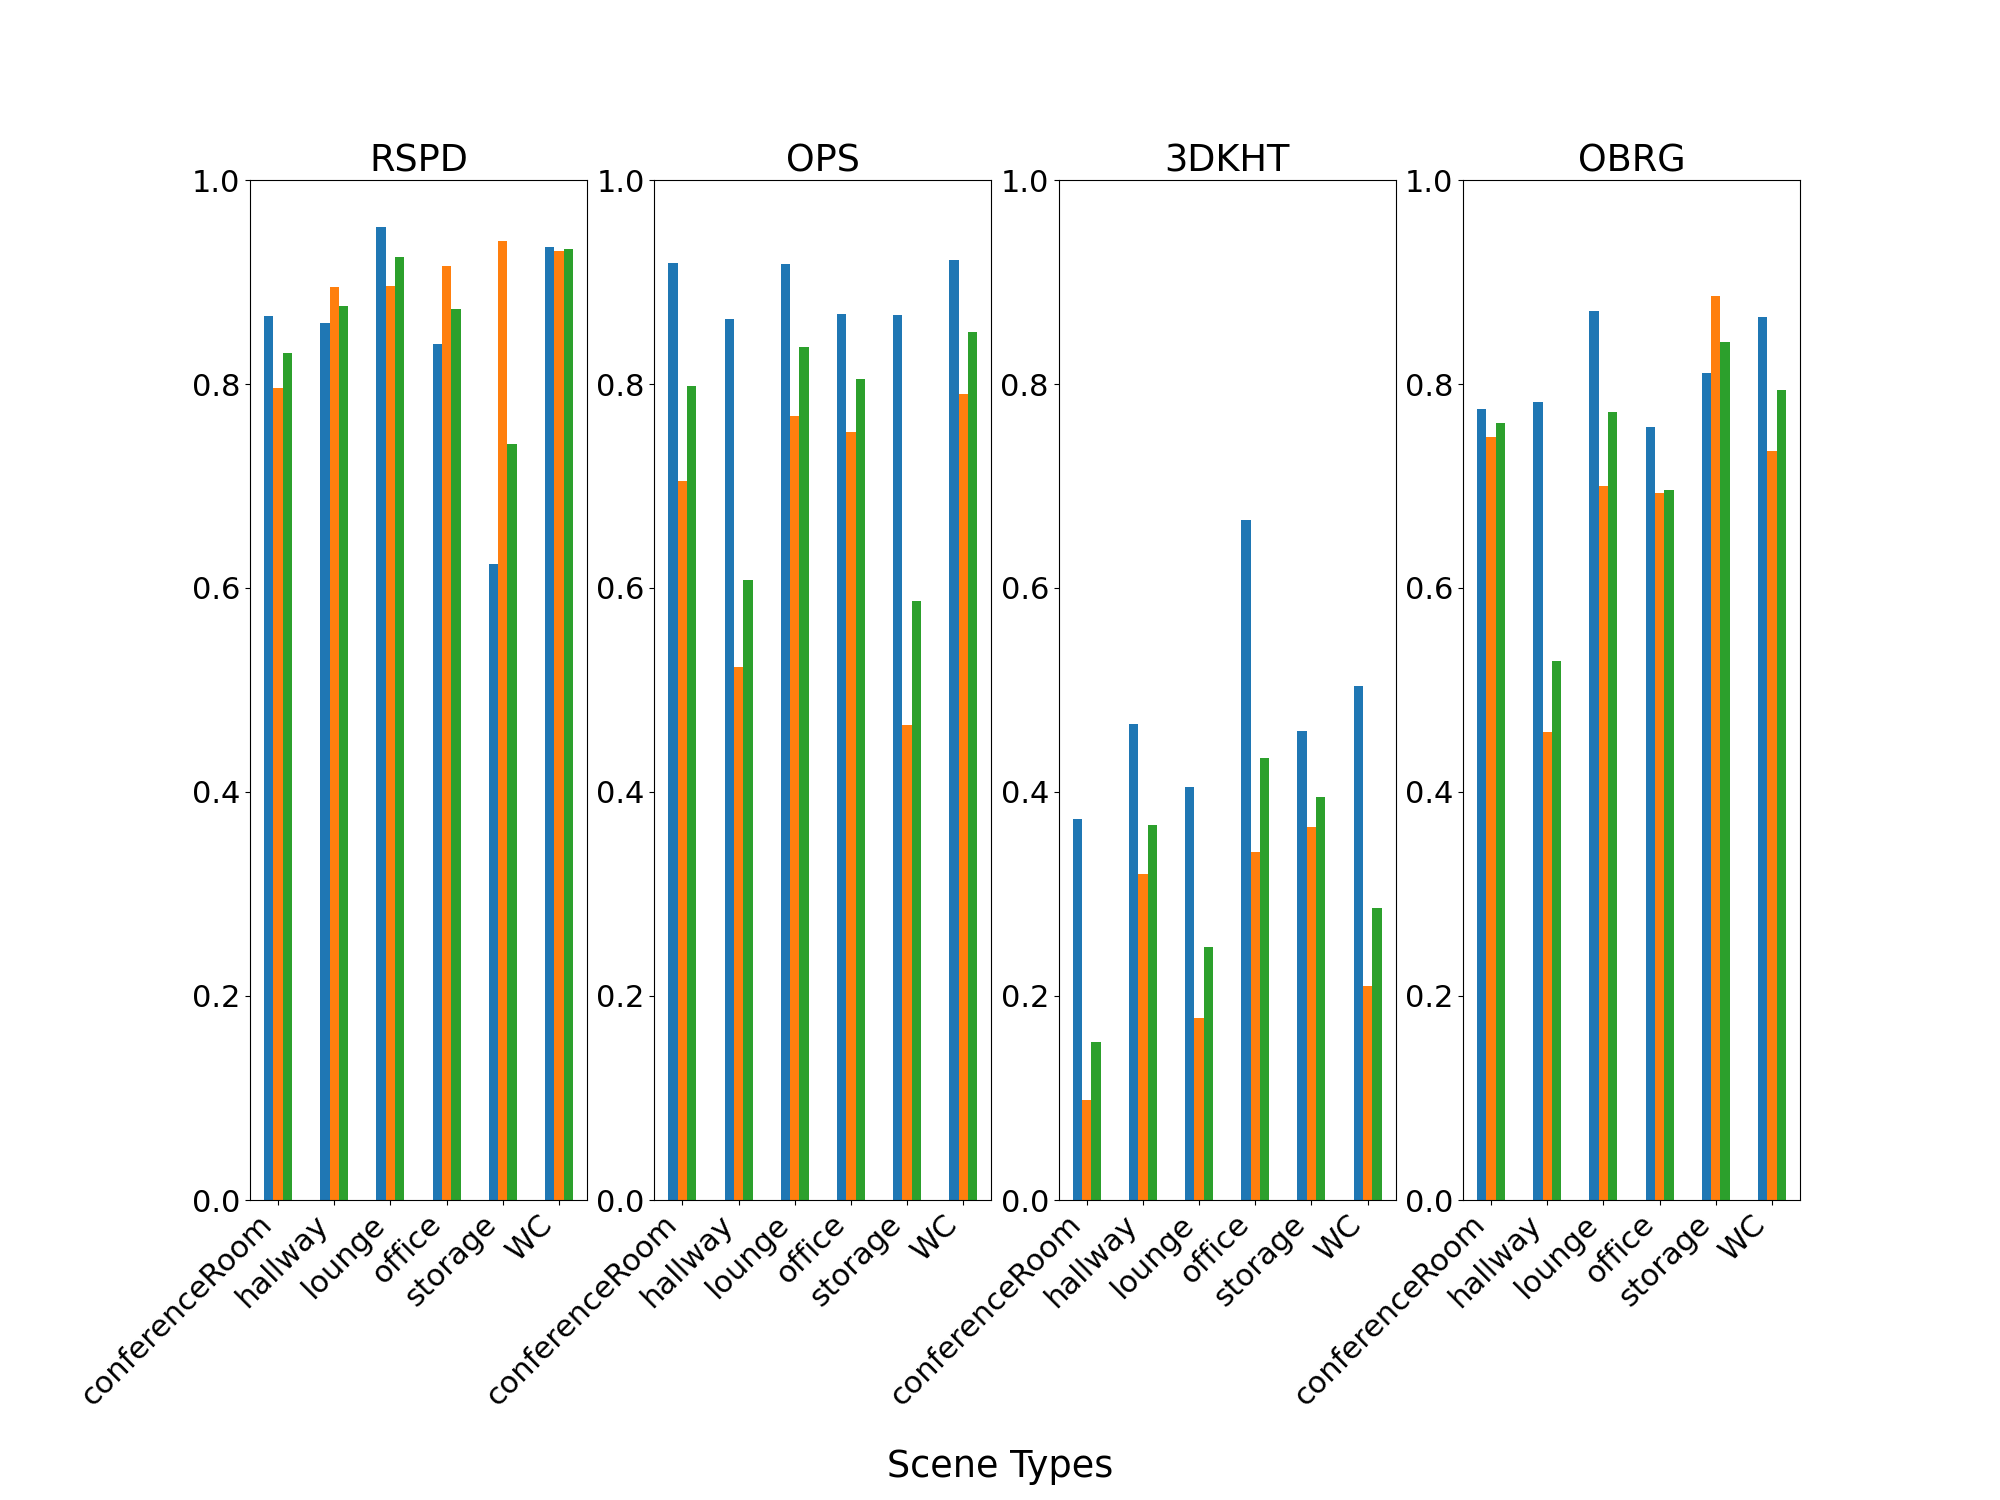
\includegraphics[width=15 cm]{images/area_3_acc.png}
    \label{fig:area3A}
    \caption[Accuracies Area 3]{Average Accuracy for each scene type of Area 3. The Precision
        is colored blue, recall is orange and the F1-score is green. }
\end{figure}


\begin{figure}[H]
    % FIXME normalize times 
    \centering
    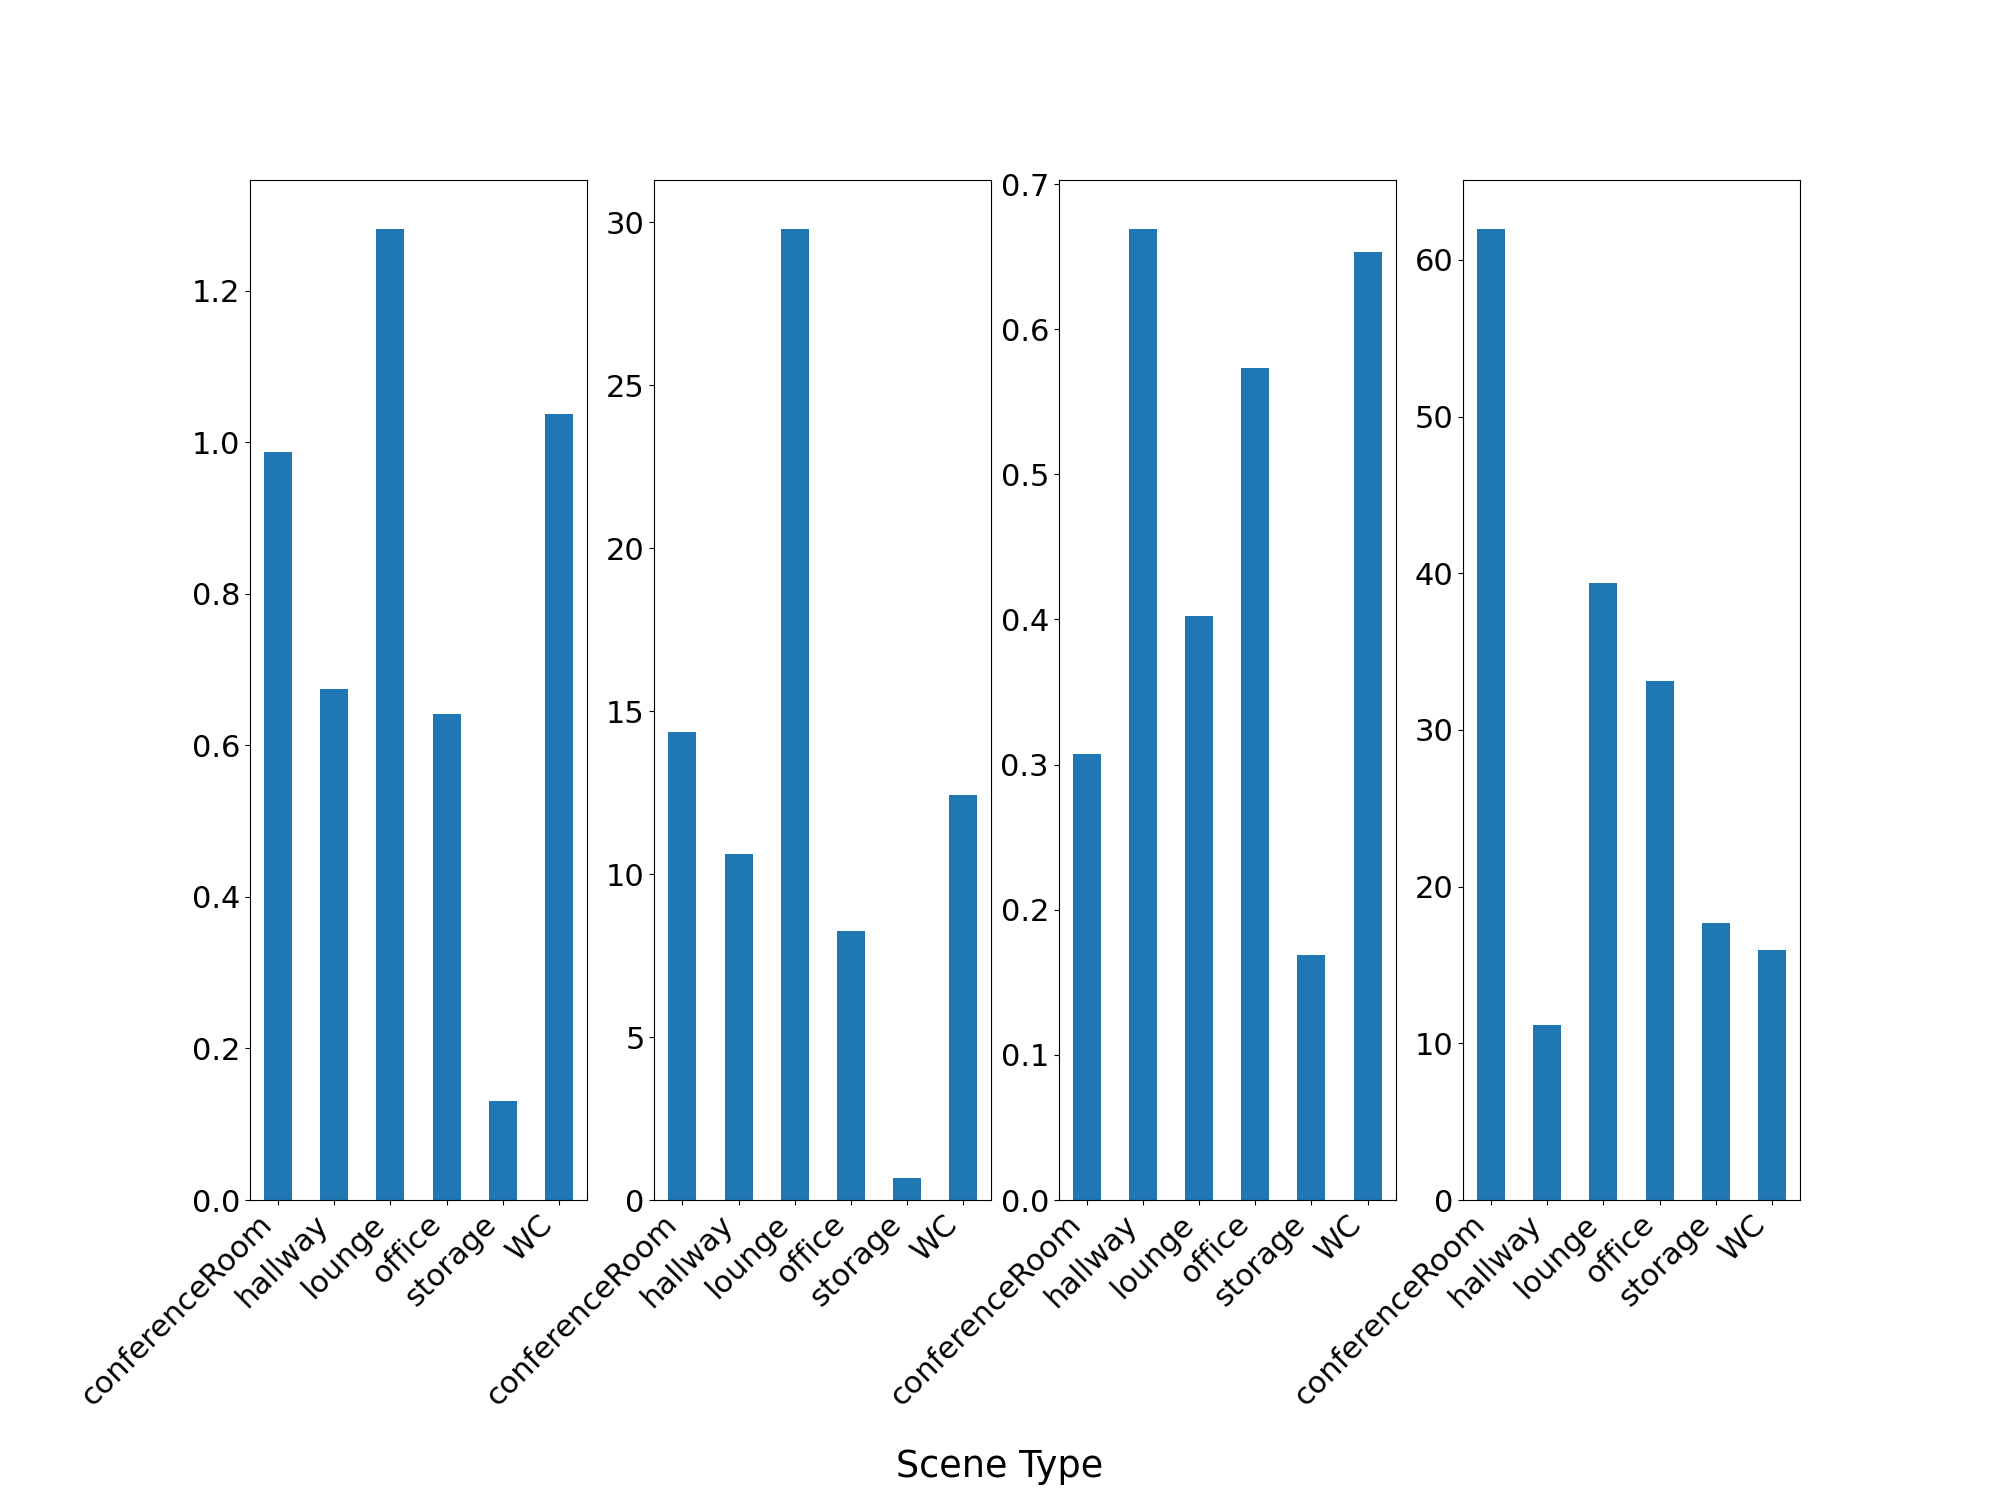
\includegraphics[width=15 cm]{images/area_3_time.png}
    \label{fig:area3T}
    \caption[Times Area 3]{Average Time per scene type of Area 3}
\end{figure}


\subsection{Area 4}

\begin{figure}[H]
    \centering
    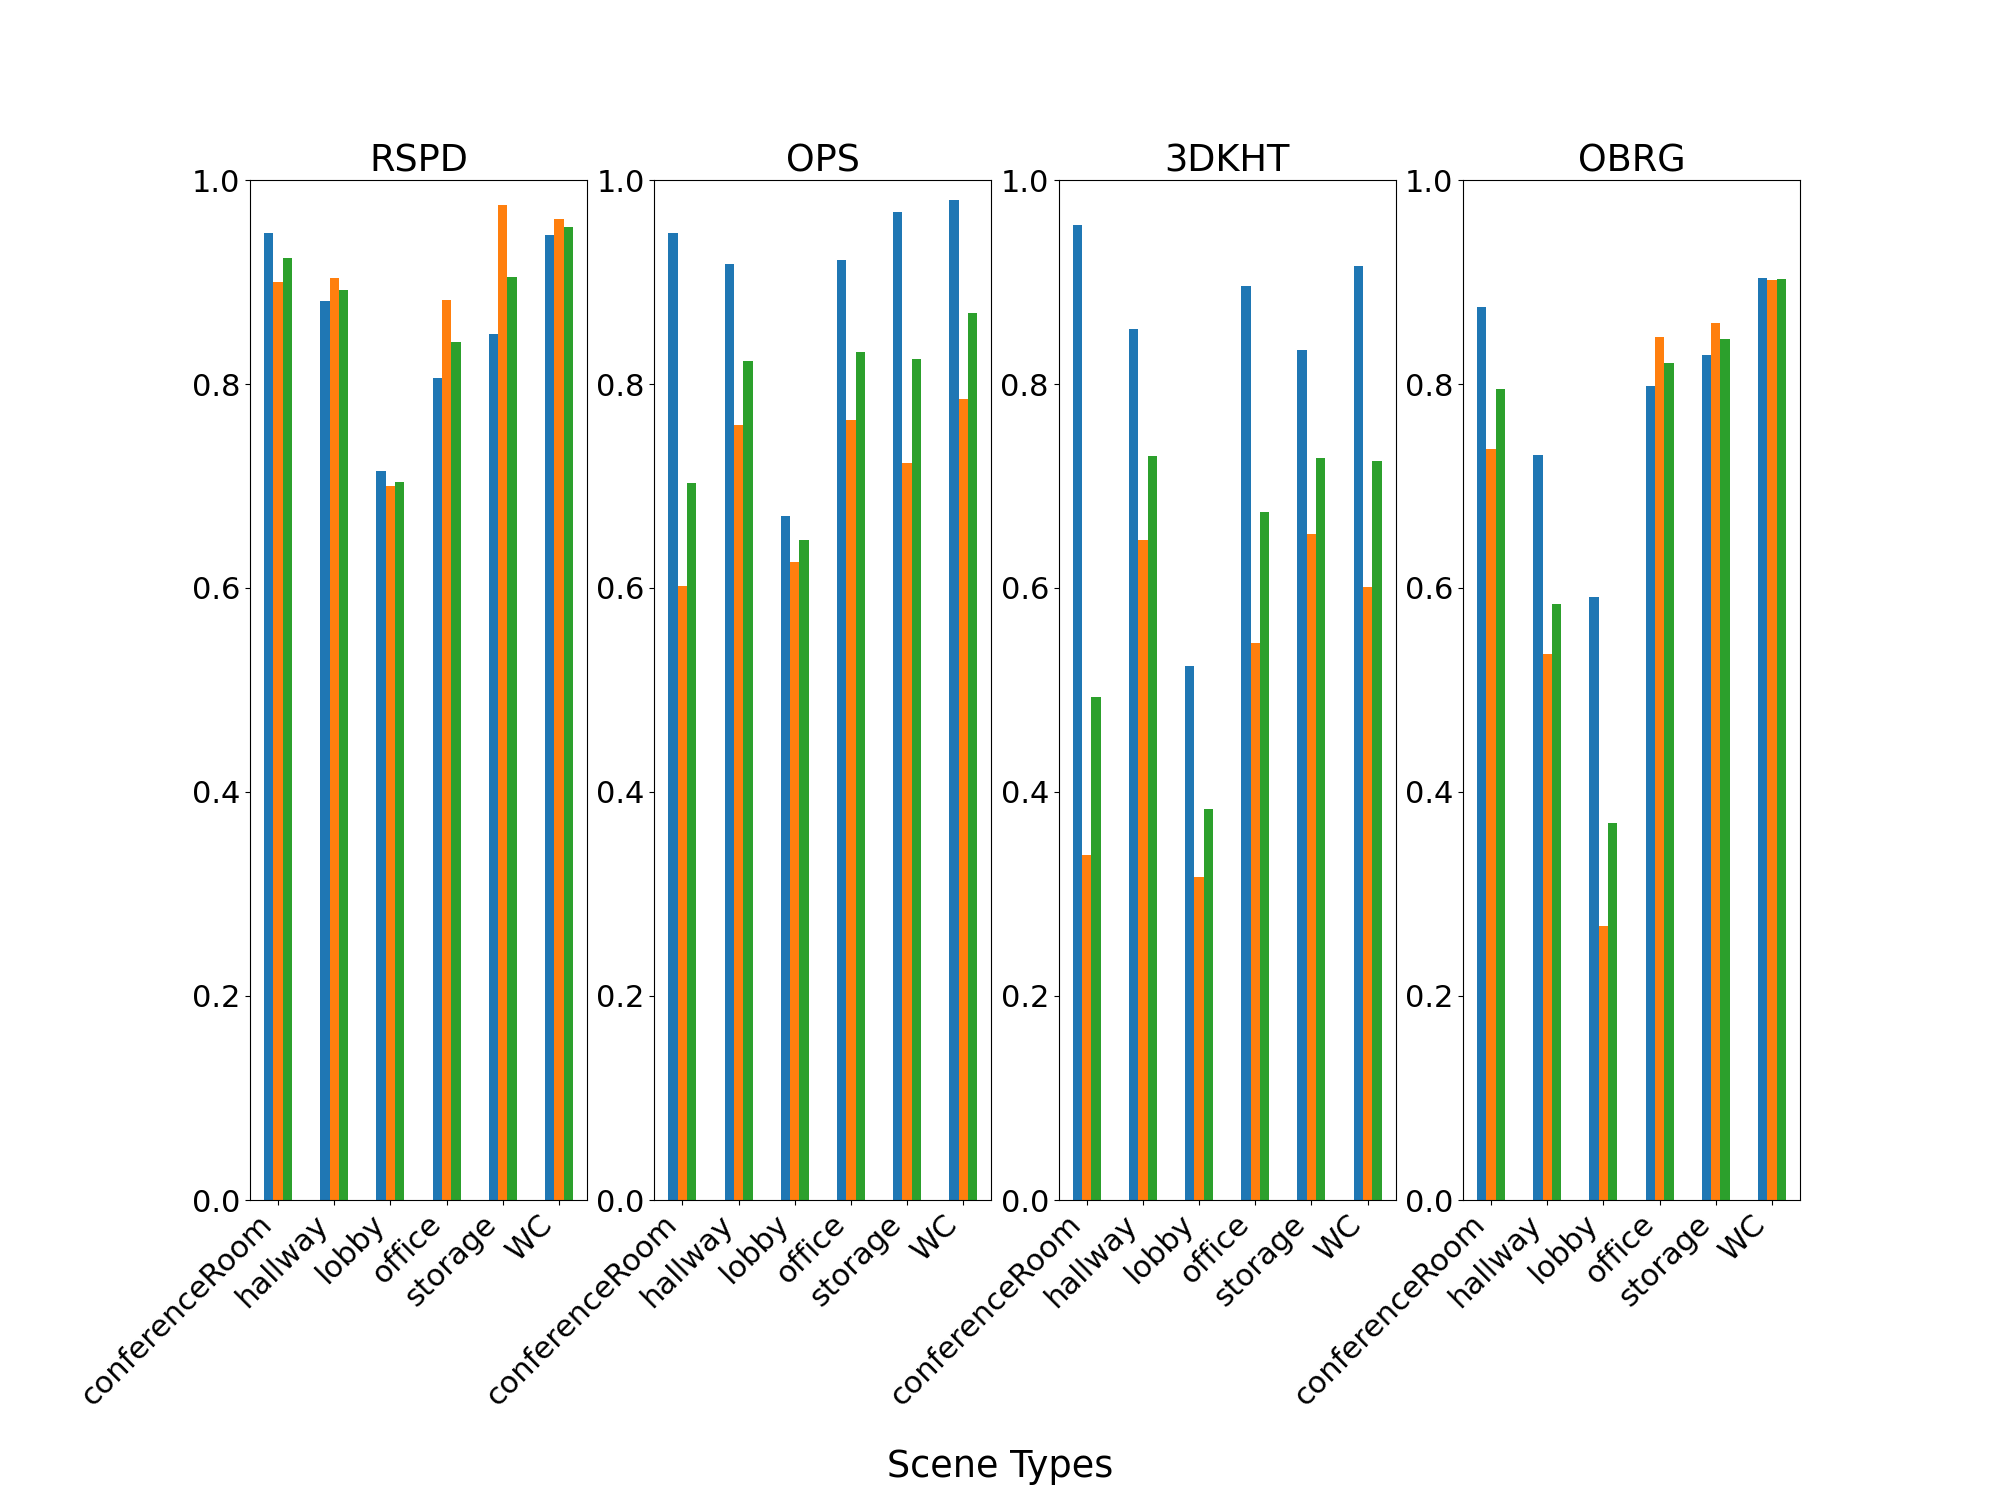
\includegraphics[width=15 cm]{images/area_4_acc.png}
    \label{fig:area4A}
    \caption[Accuracies Area 4]{Average Accuracy for each scene type of Area 4. The Precision
        is colored blue, recall is orange and the F1-score is green. }
\end{figure}

\begin{figure}[H]
    % FIXME normalize times 
    \centering
    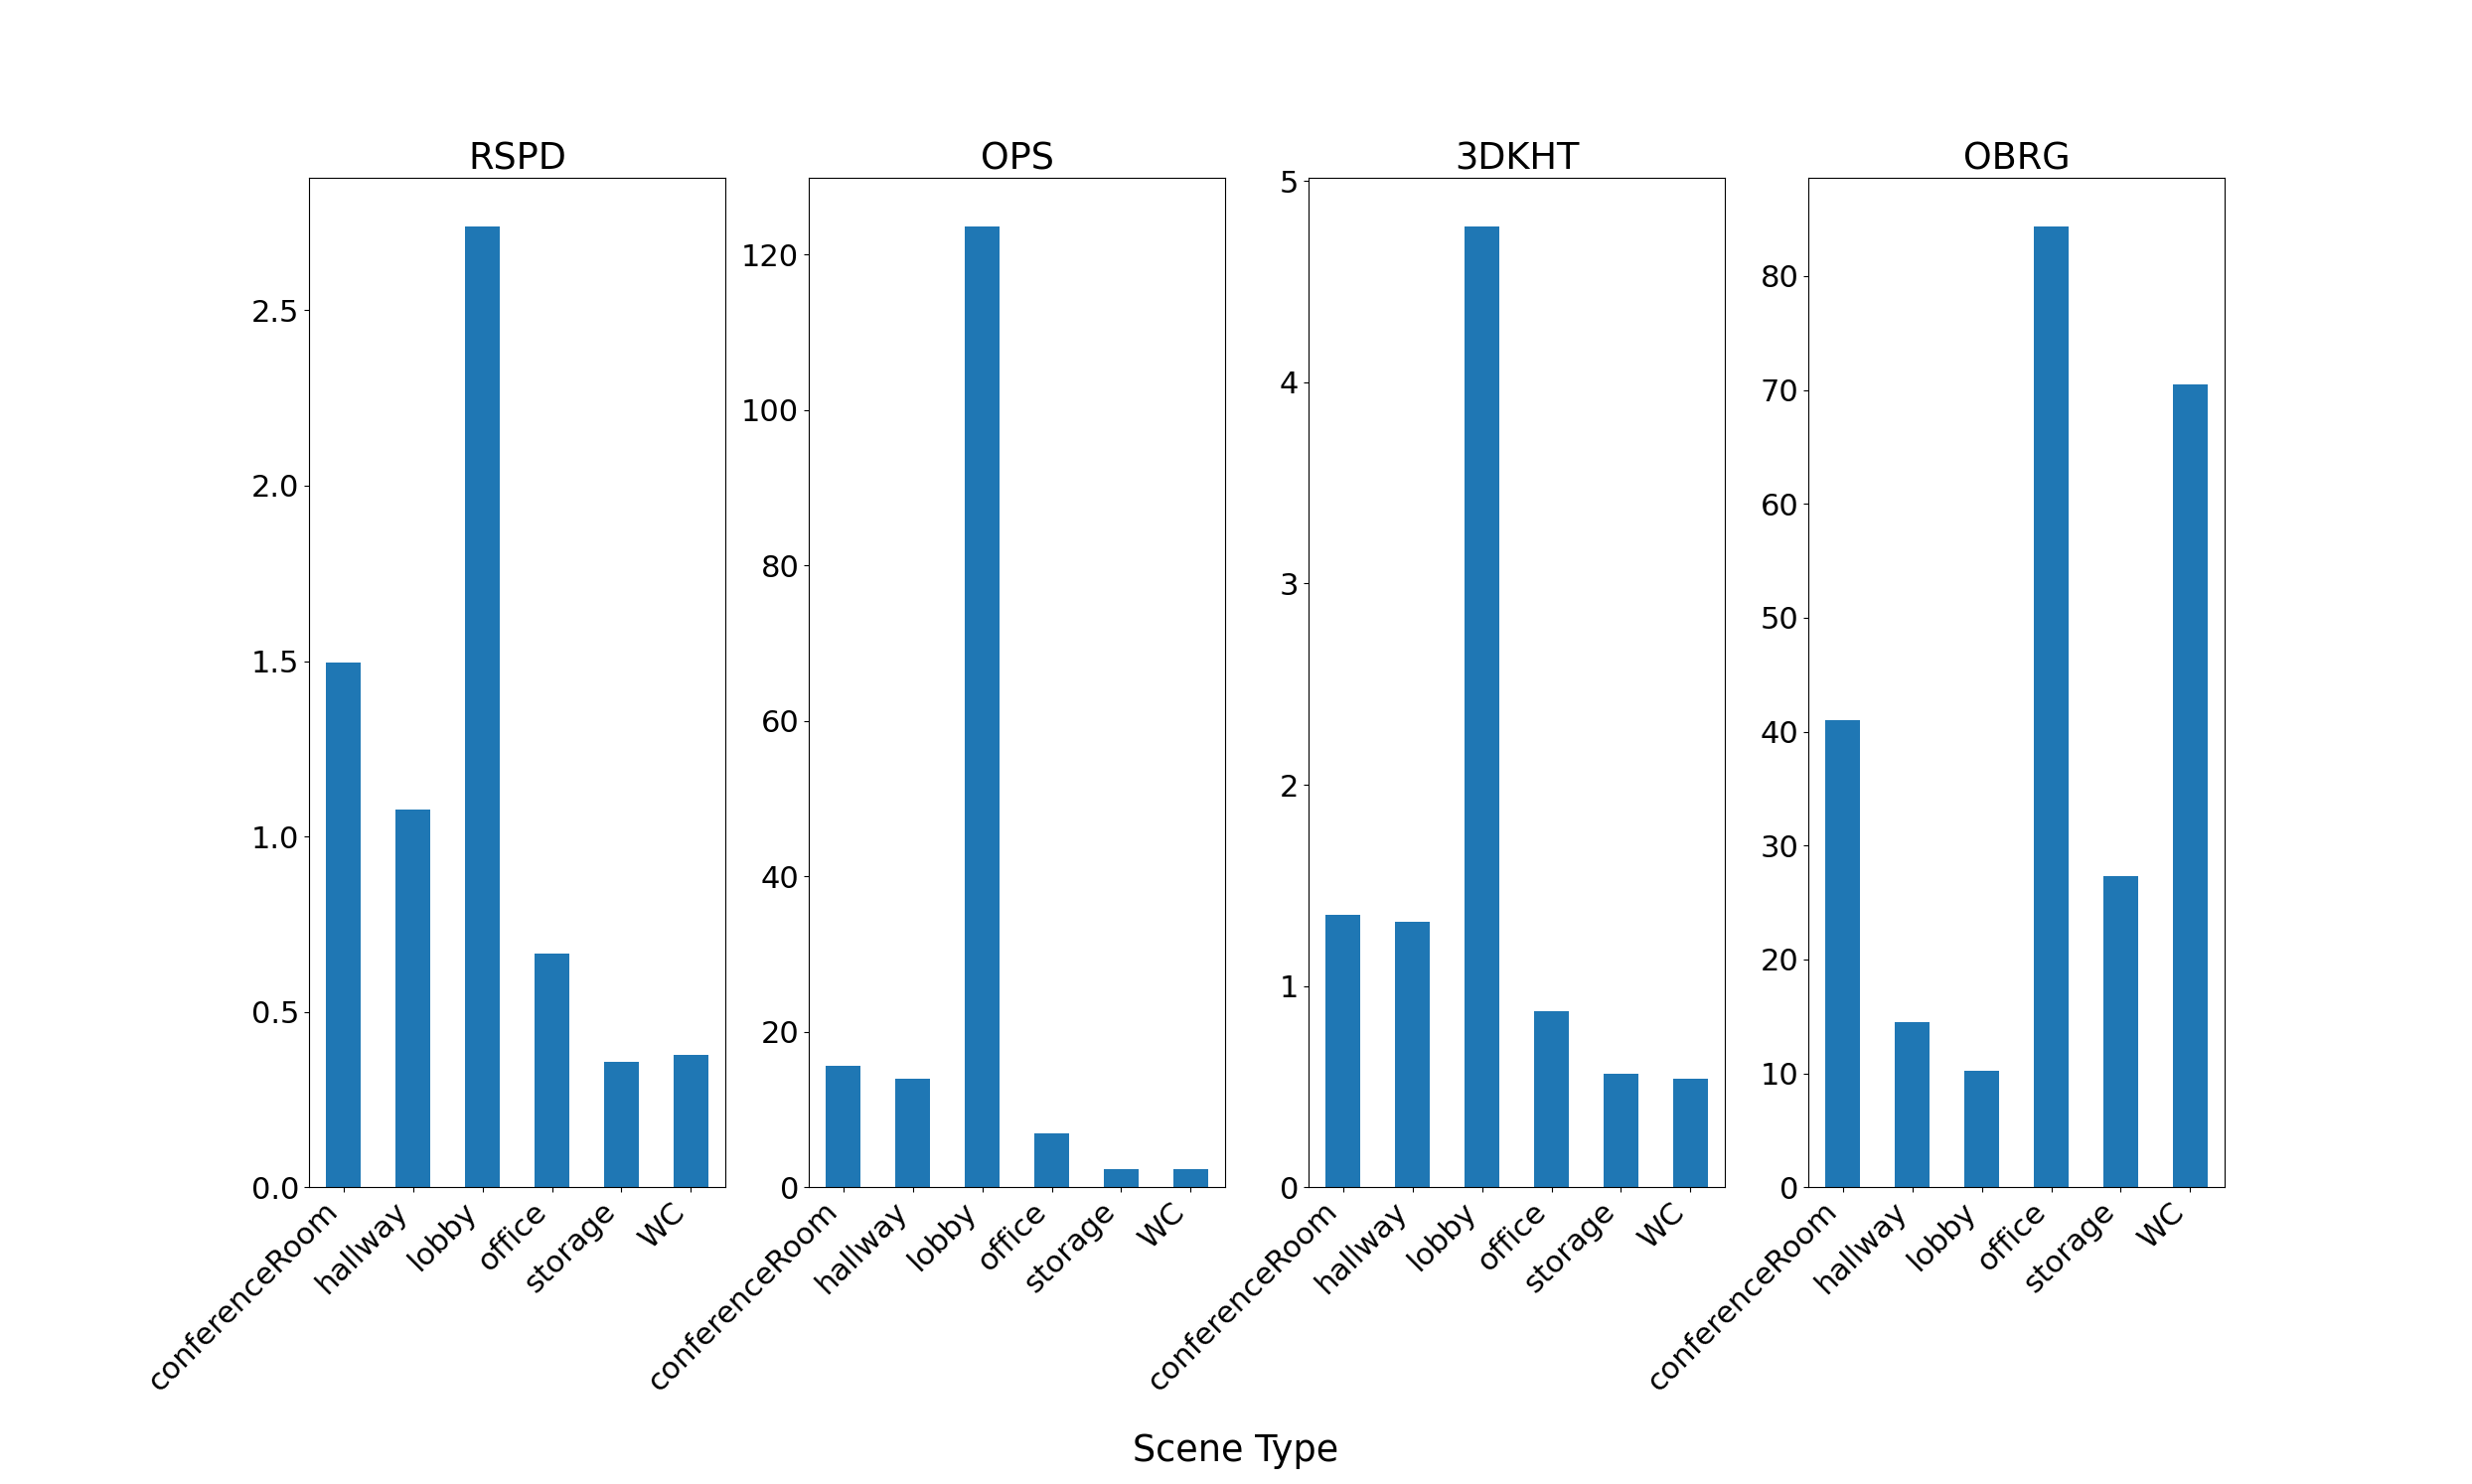
\includegraphics[width=15 cm]{images/area_4_time.png}
    \label{fig:area4T}
    \caption[Times Area 4]{Average Time per scene type of Area 4}
\end{figure}


\subsection{Area 5}

\begin{figure}[H]
    \centering
    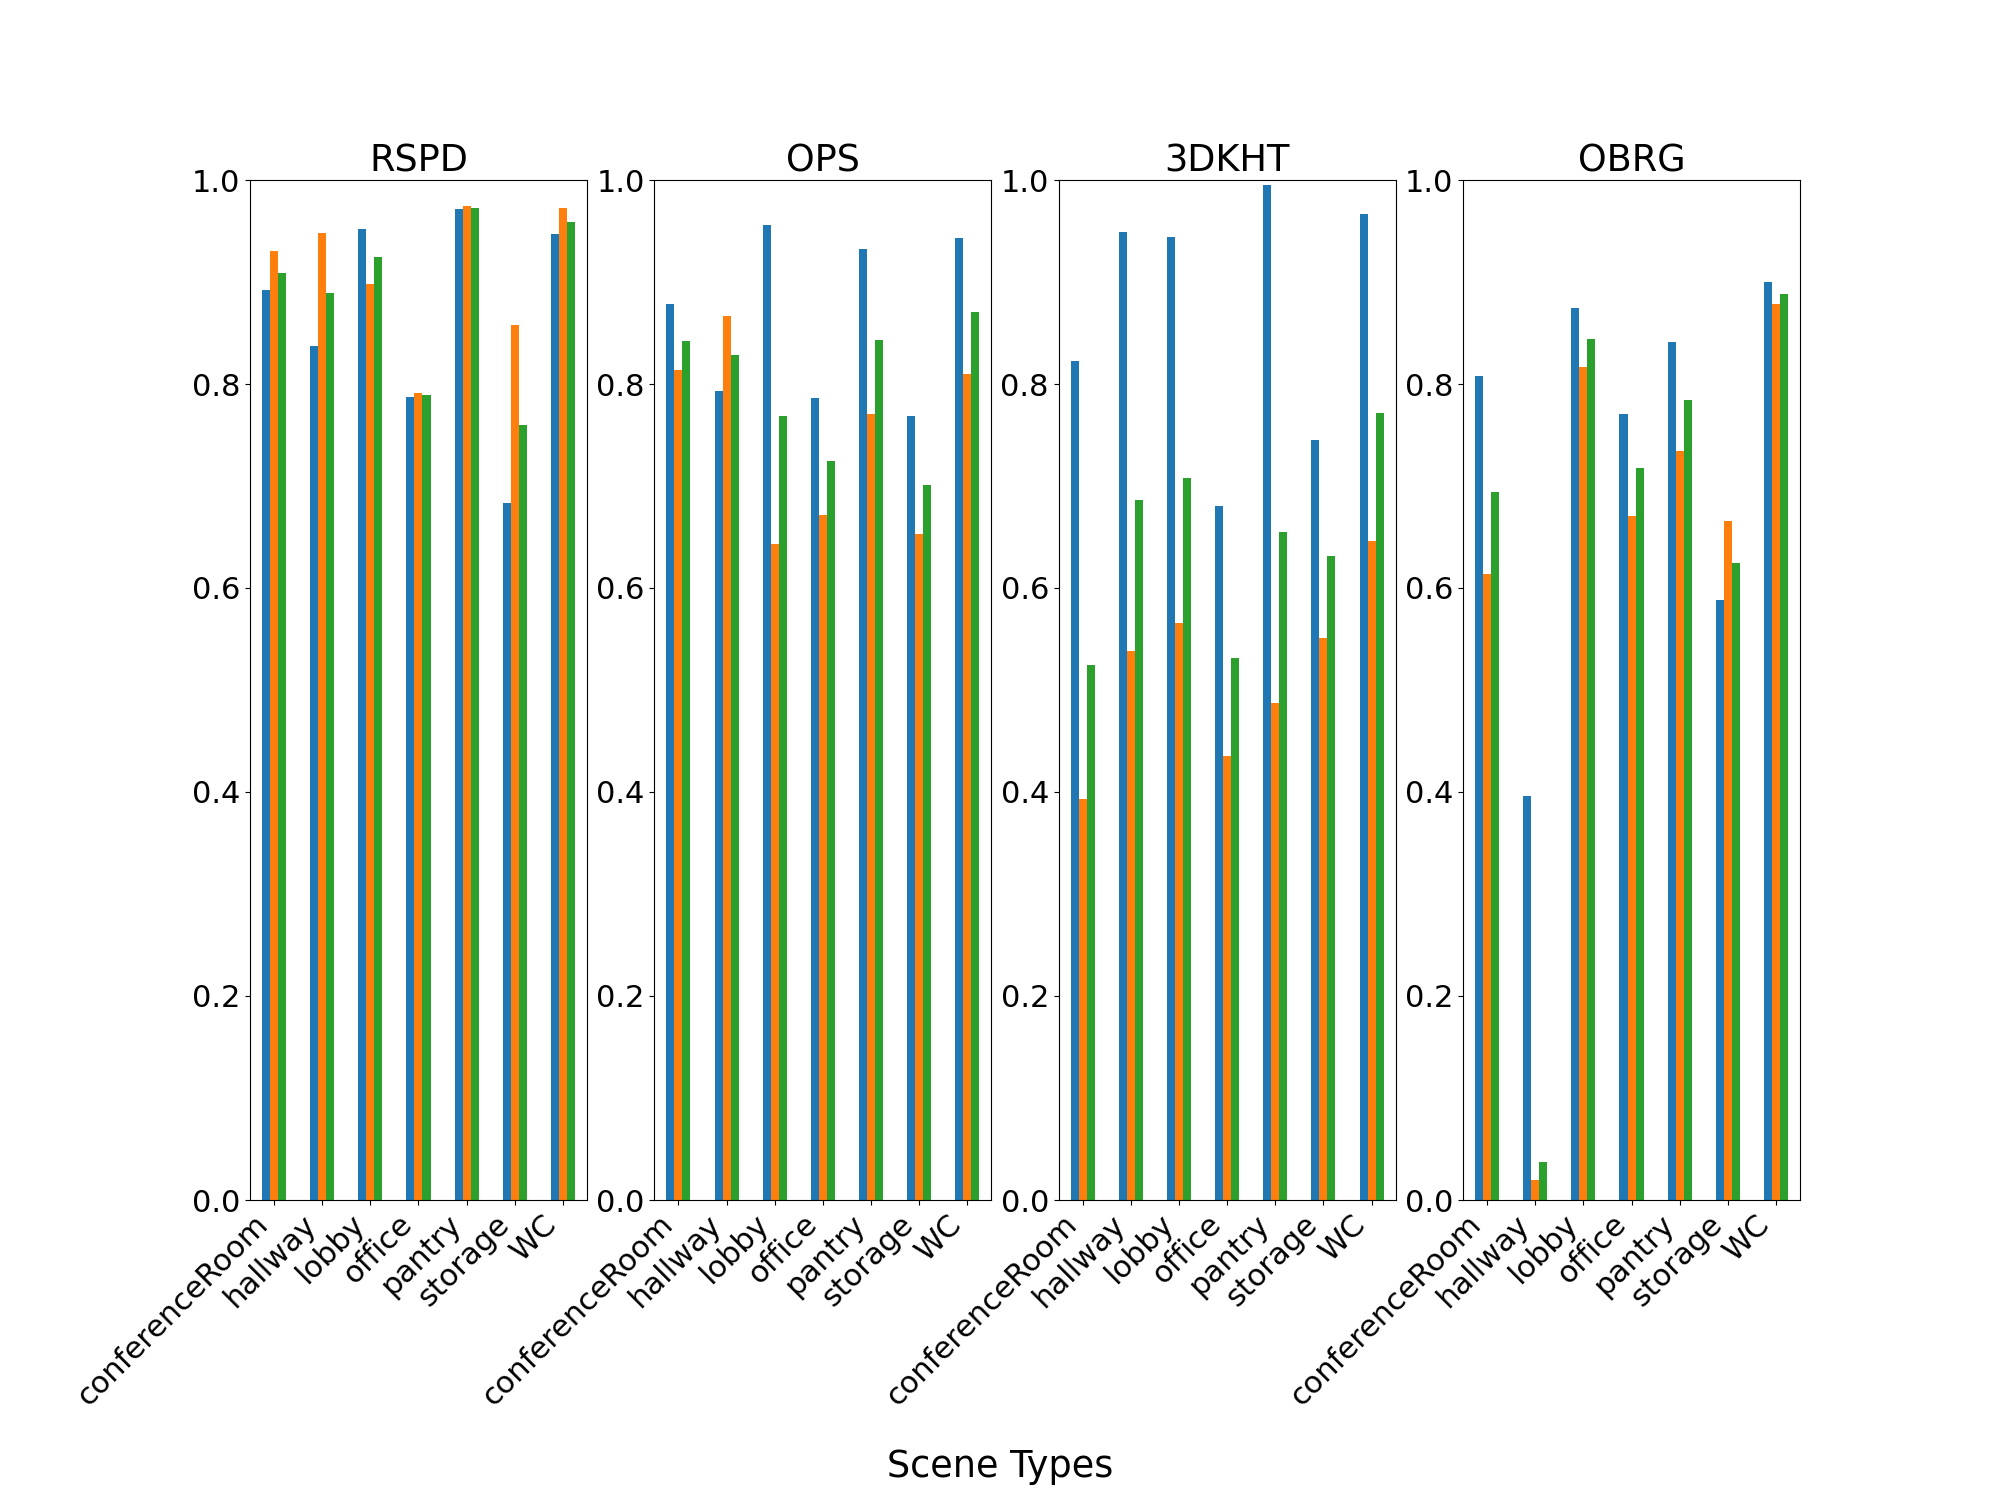
\includegraphics[width=15 cm]{images/area_5_acc.png}
    \label{fig:area5A}
    \caption[Accuracies Area 4]{Average Accuracy for each scene type of Area 5. The Precision
        is colored blue, recall is orange and the F1-score is green. }
\end{figure}


\begin{figure}[H]
    % FIXME normalize times 
    \centering
    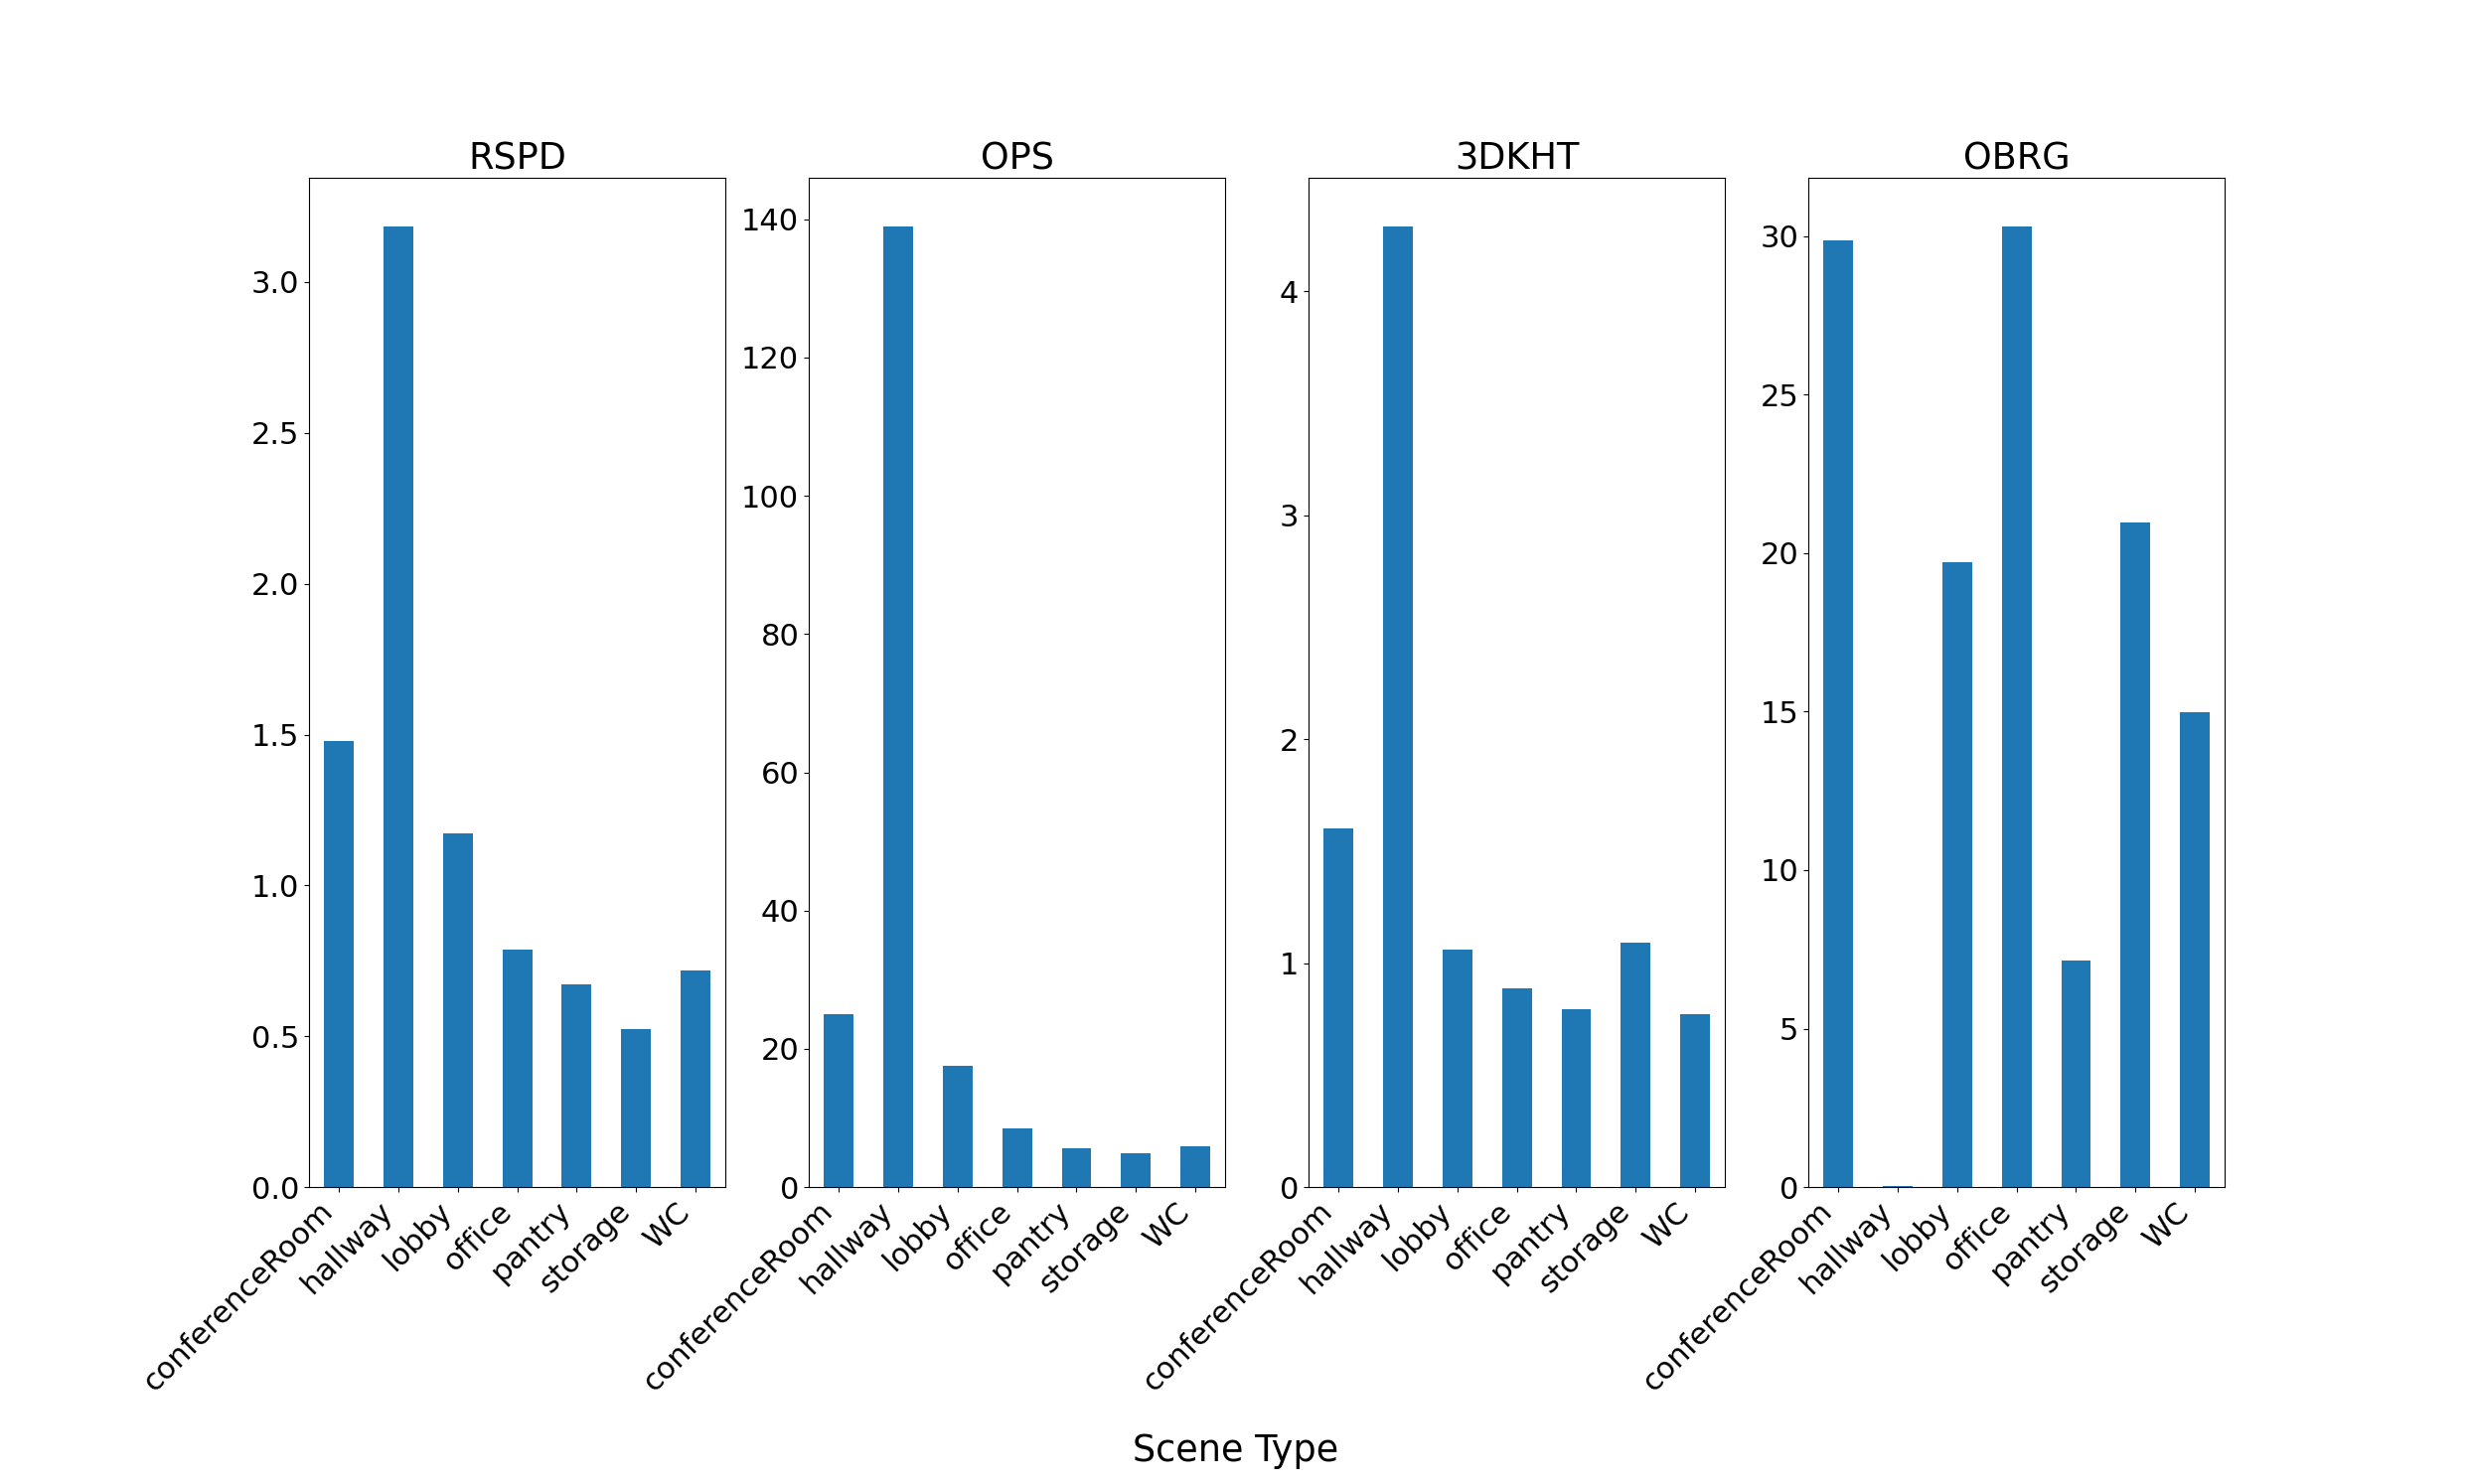
\includegraphics[width=15 cm]{images/area_5_time.png}
    \label{fig:area5T}
    \caption[Times Area 5]{Average Time per scene type of Area 5}
\end{figure}

\subsection{Area 6}

\begin{figure}[H]
    \centering
    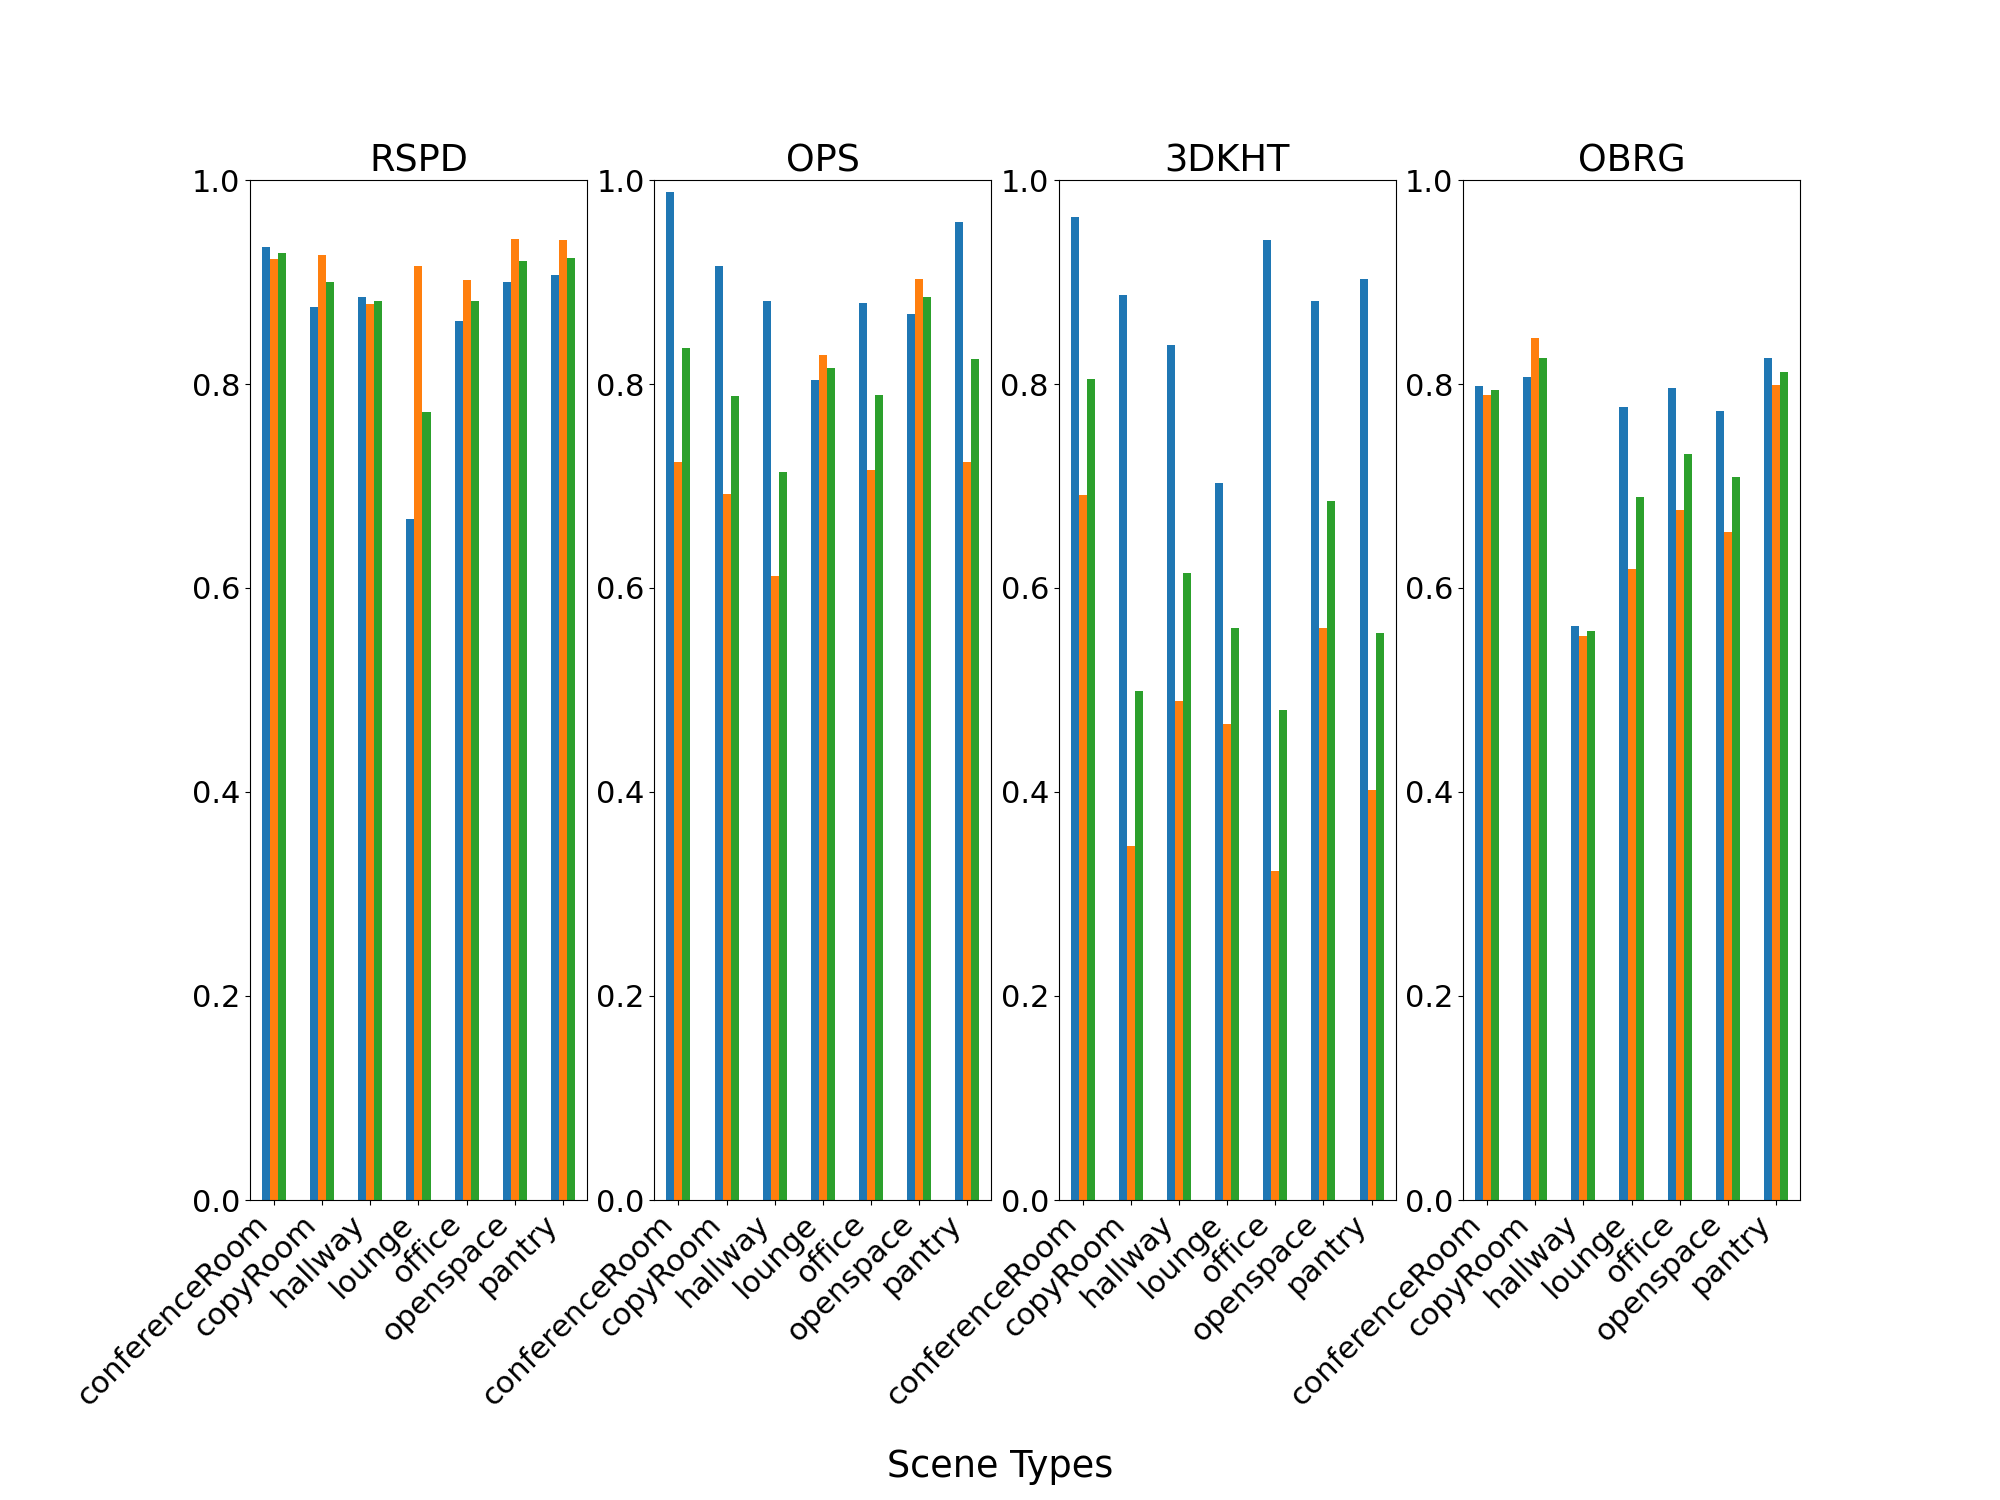
\includegraphics[width=15 cm]{images/area_6_acc.png}
    \label{fig:area6A}
    \caption[Accuracies Area 6]{Average Accuracy for each scene type of Area 6. The Precision
        is colored blue, recall is orange and the F1-score is green. }
\end{figure}


\begin{figure}[H]
    % FIXME normalize times 
    \centering
    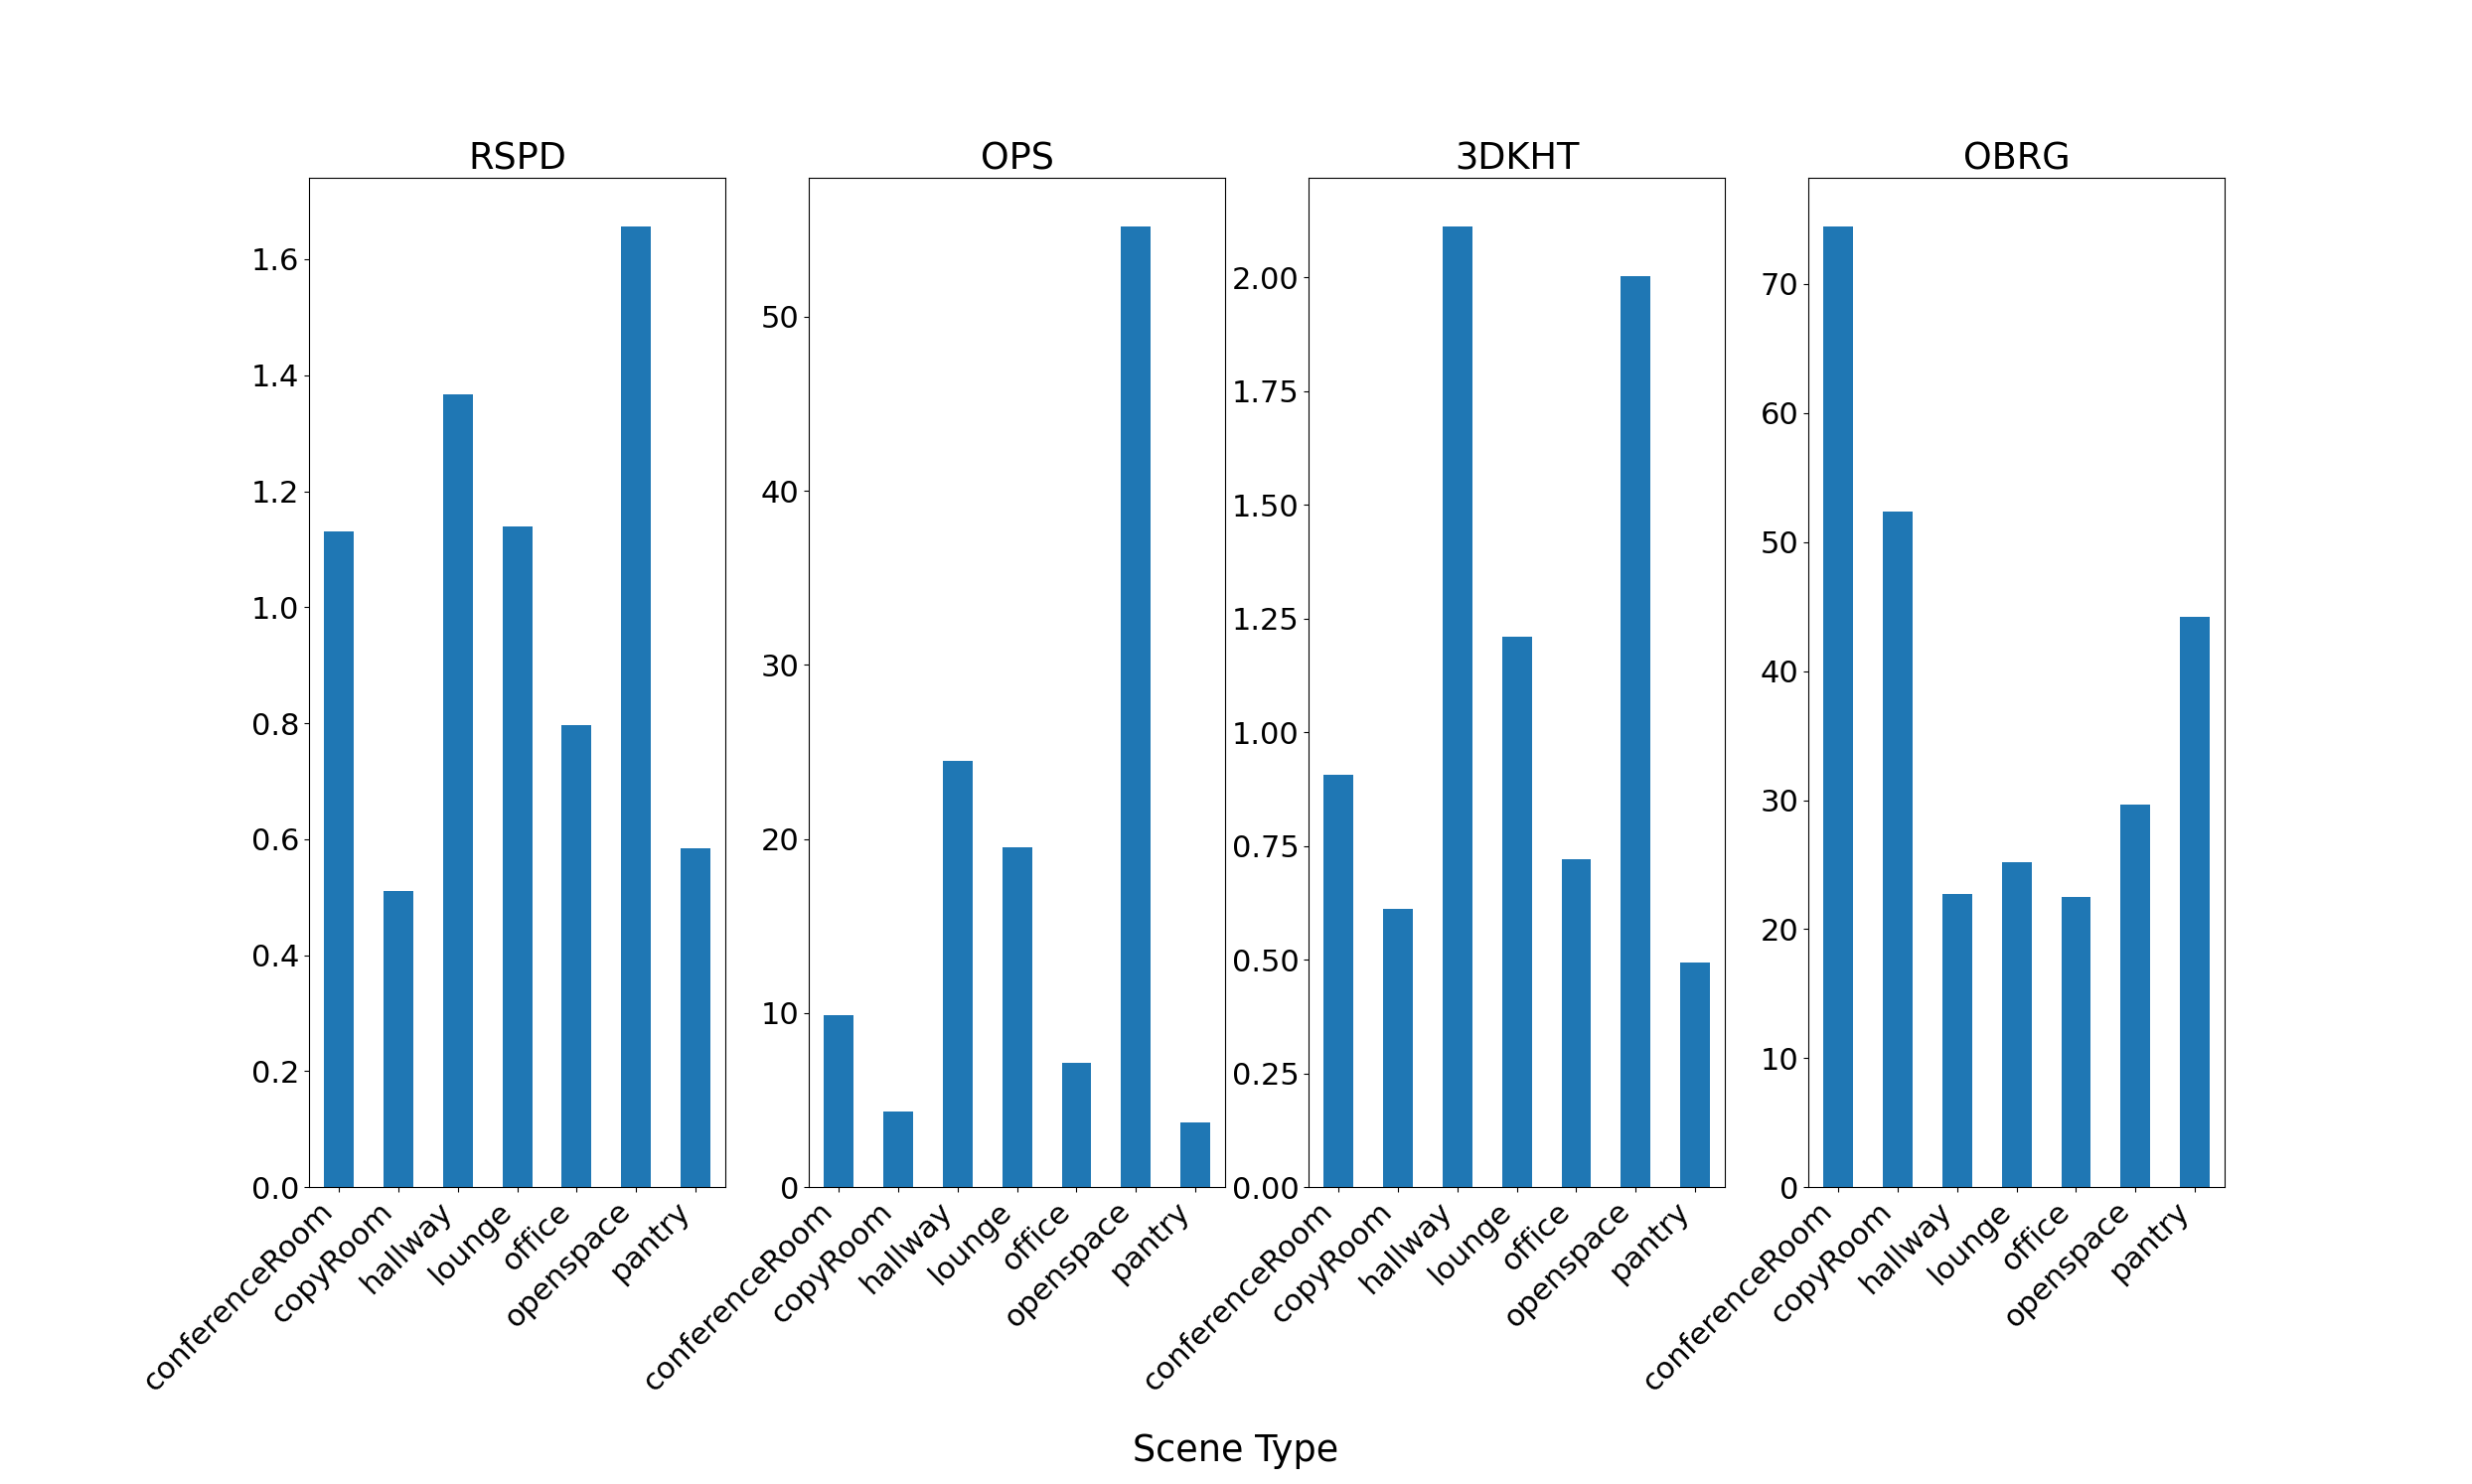
\includegraphics[width=15 cm]{images/area_6_time.png}
    \label{fig:area6T}
    \caption[Times Area 6]{Average Time per scene type of Area 6}
\end{figure}

\subsection*{Results S3DIS Experiments}
Es kristallisiert sich eindeutig heraus, dass RSPD die konsistentesten Ergebnisse hinsichtlich
Precision, Recall und F1 liefert. Diese werte sind bei OPS auch nicht schlecht, dafür ist die
berechnungszeit um ein vielfaches langsamer (~30x). 3DKHT liefert von allen Algorithmen die schlechtesten
Ergebnisse, braucht dafür im Schnitt am wenigsten zeit. Die eigen implementierung von OBRG liefert teils ergebnisse,
welche mit denen von OPS vergleichbar sind, ist dabei aber noch langsamer. Das liegt zweifelsohne an der wahl der
programmiersprache, dazu wurde nicht viel zeit in der optimierung investiert.

Statistisch gesehen sind die ergebnisse der offices und hallways am aussagekräftigsten, das liegt daran, dass davon einfach am meisten vorhanden sind.
% TODO some kind of variance? -> violin plot



\subsection{Results Real-Life Experiments}

Hier sind die Ergebnisse des dynamischen experiments.:
Es zeigt sich dass X besonders gut oder schlecht ebenen finden konnte. Wie man sich schon anhand des statischen tests denken konnte, haben OPS und OBRG zeitlich
gesehen nicht schlecht abgeschnitten.

\subsection*{Summary Experiments}
Überleitung von statisch auf dynamisch, dh. vergleich ohne, bzw. mit temporaler komponente.

Die ergebnisse der beiden experimente unterscheiden sich in folgendem punkt. Dazu sei gesagt, dass die experimente folgende übereinstimmungen haben.
Das lässt sich so erklären. Alternative gründe davon könnten diese hier sein.

Ich denke RSPD ragt heraus, da hier besonders auf noise resistenz geachtet wurde. % TODO verweis auf diverse noise tests im BG


\end{document}